% article.tex — full HBMAE journal manuscript for Nuclear Science and Engineering.
% Target: NSE regular article, ~40-44 pp double-spaced, MS-student-accessible.
% Compile: pdflatex + bibtex (references.bib in same directory).

\documentclass[12pt]{article}
\usepackage[margin=1in]{geometry}
\usepackage[doublespacing]{setspace}
\usepackage{amsmath,amssymb,amsthm}
\usepackage{mathtools}
\usepackage{graphicx}
\usepackage{hyperref}
\usepackage[round,authoryear]{natbib}
\usepackage{algorithm,algpseudocode}
\usepackage{booktabs}
\usepackage{xspace}
\usepackage{siunitx}
\usepackage[most]{tcolorbox}      % for "tutorial boxes"
\usepackage{caption}
\captionsetup{font=small,labelfont=bf}

% Theorem environments (full proofs in Appendix A; main text uses lightweight 'result')
\theoremstyle{plain}
\newtheorem{theorem}{Theorem}
\newtheorem{lemma}[theorem]{Lemma}
\newtheorem{proposition}[theorem]{Proposition}
\newtheorem{corollary}[theorem]{Corollary}
\theoremstyle{definition}
\newtheorem{definition}{Definition}
\newtheorem{assumption}{Assumption}
\theoremstyle{remark}
\newtheorem{remark}{Remark}

% Tutorial-box environment: shaded box with title for pedagogical asides.
\newtcolorbox{tutorialbox}[1]{
  colback=blue!4, colframe=blue!50!black,
  fonttitle=\bfseries\small, title=#1,
  enhanced, breakable,
  boxrule=0.4pt, arc=2pt, left=4pt, right=4pt, top=2pt, bottom=2pt,
  before skip=6pt, after skip=6pt,
}

% "Common pitfall" box: distinct color for warnings.
\newtcolorbox{pitfall}[1]{
  colback=red!3, colframe=red!50!black,
  fonttitle=\bfseries\small, title=Common pitfall: #1,
  enhanced, breakable,
  boxrule=0.4pt, arc=2pt, left=4pt, right=4pt, top=2pt, bottom=2pt,
  before skip=6pt, after skip=6pt,
}

% Notation shortcuts (consistent with methods.tex)
\newcommand{\eS}{\ensuremath{e_{\mathrm{s}}^{-}}\xspace}
\newcommand{\Clt}{\ensuremath{\mathrm{Cl}_2^{\bullet-}}\xspace}
\newcommand{\Cltdiss}{\ensuremath{\mathrm{Cl}_{2,\,\mathrm{diss}}}\xspace}
\newcommand{\HBMAE}{HBMAE\xspace}
\newcommand{\Ea}{E_a}
\renewcommand{\d}{\mathrm{d}}
\newcommand{\R}{\mathbb{R}}
\newcommand{\E}{\mathbb{E}}
\newcommand{\dotp}[2]{\langle #1, #2 \rangle}
\newcommand{\norm}[1]{\lVert #1 \rVert}

\title{\bfseries Hierarchical Bayesian Mechanism-Adequacy Estimation for Molten Salt
       Radiolysis Networks: A Practical Framework with Validation Against the
       Pulse-Radiolysis Literature}

\author{M.\ Tanore-Tamales \\
        \small Idaho National Laboratory, Idaho Falls, ID 83415, USA \\
        \small \texttt{mauricio.tanoretamales@inl.gov}}

\date{\today}

\begin{document}
\maketitle

\begin{abstract}
\noindent
Radiolysis kinetic networks for molten salt reactors must be calibrated against
heterogeneous experimental data spanning fourteen orders of magnitude in time,
multiple laboratory facilities with documented systematic biases, multiple
chemically-distinct host salts, and one-sided detection limits.  No published
Bayesian-calibration framework simultaneously addresses all five of these features.
We introduce \HBMAE\ (Hierarchical Bayesian Mechanism-Adequacy Estimation), a
framework that composes (i)~a chemistry-constrained spike-and-slab prior on
reaction inclusion, (ii)~a hierarchical Arrhenius layer coupling shared
elementary reactions across salts, (iii)~a Godambe-balanced composite likelihood
spanning transient time-series, scalar rate constants, censored detection
bounds, and derived Arrhenius pairs, (iv)~a parametric model-discrepancy term
robust to the Brynjarsd\'ottir--O'Hagan identifiability pathology, and
(v)~explicit facility-effect bias terms with gauge-fixing.  We prove six
theorems characterizing well-posedness, posterior consistency, asymptotic bias,
and identifiability of the framework, and we benchmark \HBMAE\ against four
state-of-the-art comparator methods on the published Iwamatsu--Horne
pulse-radiolysis data set and the Phillips~2022 Molten Chloride Fast Reactor
detection-limit benchmark.  \HBMAE\ recovers literature Arrhenius parameters
within published~$\sigma$ for all four calibrated reactions, identifies a
Pikaev--Iwamatsu inter-laboratory bias of factor~$0.035$ that has long been a
qualitative concern in the radiation-chemistry community, and yields a censored
Bayes-factor of~$\sim 10^{138}$ in favor of chloride kernels that include the
\mbox{U(III)/U(IV)} redox sink, against kernels that omit it.  We extend the
framework to a predictive-for-any-element setting via a meta-hierarchical
chemistry-feature regression on nine metals across five host matrices, a
PSIS-LOO network-selection demonstration, and a calibrated fluoride
F$_2$-production kernel anchored to the Davis~2022 G-values and the
Toth--Felker~1990 recombination data.  The framework is designed to be
accessible to graduate students entering molten salt
radiation-chemistry; we include tutorial boxes, worked examples, an open-source
implementation, and suggested exercises.
\end{abstract}

\noindent\textbf{Keywords:}
molten salt reactor;
radiolysis;
chemical kinetic network;
Bayesian model adequacy;
hierarchical inference;
uncertainty quantification;
LiCl--KCl eutectic;
NaCl--UCl$_3$.

\bigskip

% =============================================================================
\section{Introduction}\label{sec:intro}
% =============================================================================

The radiation chemistry of molten salts has moved from background concern to
front-line engineering question over the past decade as the molten salt reactor
(MSR) has re-emerged as a leading advanced-fission concept.  Concept studies for
the Molten Chloride Fast Reactor \citep{TerraPower2021}, the Fluoride-Salt-Cooled
High-Temperature Reactor \citep{Forsberg2020}, and chloride-fueled and
fluoride-fueled fast spectrum systems share a common requirement:  defensible,
validated predictions of how the salt's chemical inventory evolves under
radiation, on time scales spanning nanoseconds (radiolytic transient species)
through years (cumulative redox shifts and gas-phase product accumulation).
Below detection limits, those predictions are required for plant-safety
analyses; above detection limits, they govern off-gas system design and
corrosion management.

The pulse-radiolysis literature that supplies the underlying rate constants is
now substantial.  The Brookhaven Linac Electron Accelerator Facility (LEAF)
program has produced quantitative kinetics for the solvated electron
\eS\ and the dichlorine radical anion \Clt\ in molten LiCl--KCl eutectic
\citep{Iwamatsu2022}, for chromium-mediated electron transfer
\citep{Iwamatsu2026}, for iodide perturbation \citep{Conrad2023}, for
neodymium speciation \citep{CastroBaldivieso2026}, and for the first
actinide rate constants in chloride media~\citep{Rotermund2024}.
Earlier Soviet-era work \citep{Pikaev1982,Makarov1982,Hagiwara1987}
established the basic transient inventory across the alkali halide series,
and recent ab initio molecular dynamics simulations~\citep{KristoffersenMetiu2018}
provide thermodynamic-feasibility anchors for the redox sub-network.
Steady-state fluorine-gas yields from gamma-irradiated LiF, BeF\textsubscript{2},
UF\textsubscript{4}, ThF\textsubscript{4}, and FLiBe powders have been recently
quantified \citep{Davis2022}, complementing the early Toth--Felker recombination
measurements~\citep{Toth1990}.  In the chloride-salt nuclear-fuel context,
Phillips and coworkers \citep{Phillips2022} reported the first long-duration
gamma-irradiation of \mbox{NaCl-UCl\textsubscript{3}} salt with no detectable
Cl\textsubscript{2} above approximately \SI{1000}{ppm}.

The methodological problem of \emph{combining} these heterogeneous data sources
into a predictive radiolysis model has lagged the experimental progress, and
that gap is the subject of this paper.  Existing Bayesian-calibration frameworks
were developed for single-laboratory, single-modality data sets, and they are
not well-matched to the radiolysis problem in five concrete ways.

\begin{enumerate}
\item \emph{Time-scale heterogeneity.}  Pulse-radiolysis transients evolve over
nanoseconds; chronic-irradiation gas accumulation evolves over months.  The
ratio is fourteen orders of magnitude.  A single stiff-ODE forward solver
cannot reach both ends without singular-perturbation reduction.
\item \emph{Observation modality heterogeneity.}  Different experimental
campaigns report different observable types: dense absorbance time-series,
scalar rate constants with quoted~$\sigma$, derived Arrhenius
$(\log A, \Ea)$ pairs, and one-sided censored detection limits.  Treating
these as exchangeable Gaussian observations is incorrect for censored data
and yields imbalanced posterior contraction across the others.
\item \emph{Cross-laboratory systematic bias.}  The Pikaev microsecond pulse
radiolysis of the 1980s and the Iwamatsu picosecond LEAF data of the 2020s
disagree by an order of magnitude on rate constants for ostensibly the same
reaction.  Iwamatsu and coworkers have argued qualitatively that Pikaev's
time-resolution introduced a systematic bias \citep{Iwamatsu2022}; no
published framework formalizes this as an identifiable parameter.
\item \emph{Cross-salt mechanistic transfer.}  The elementary reaction
$\eS+\mathrm{M}^{n+}\to\mathrm{M}^{(n-1)+}$ has been measured in NaCl, KCl,
LiCl--KCl, and ZnCl\textsubscript{2} hosts.  Activation parameters differ
across hosts in chemically-interpretable ways (Marcus-type solvent
reorganization), but no published framework uses these as coupled
observations of a shared intrinsic chemistry.
\item \emph{Network topology constraints.}  Mass and charge balance constrain
the feasible set of reaction-inclusion vectors~$\gamma$ to a strict subset of
$\{0,1\}^R$; reaction networks that violate these conservation laws are
unphysical.  Existing spike-and-slab Bayesian network-inference frameworks
\citep{GalagaliMarzouk2015,GalagaliMarzouk2019} place positive prior mass on
the infeasible region and pay a corresponding mixing penalty.
\end{enumerate}

This paper introduces \HBMAE, a Bayesian framework that composes five
ingredients to address these five gaps.  Each ingredient has well-established
precedent in the broader uncertainty-quantification literature; the
contribution of the paper is the \emph{synthesis} that targets molten-salt
radiation chemistry specifically, together with the theorems characterizing
when the synthesis is well-defined and identifiable, and the empirical
validation against four published data sources.

The paper is written for a reader at the early graduate-student level.  No
prior exposure to Bayesian inference, posterior computation, or model adequacy
is assumed.  Section~\ref{sec:background} develops the necessary mathematical
background from first principles, with worked examples in radiation-chemistry
notation, and includes tutorial boxes on prior choice, posterior interpretation,
Markov chain Monte Carlo, and model adequacy.  Section~\ref{sec:sota} surveys
the four existing methodological approaches against which \HBMAE\ is
compared.  Section~\ref{sec:framework} presents the framework as a sequence of
five compositional layers, each motivated by one of the five gaps above.
Section~\ref{sec:theorems} states the six theorems and four propositions, with
plain-language interpretations in the main text; the formal proofs are
deferred to Appendix~A.  Sections~\ref{sec:worked1} and~\ref{sec:worked2}
present two pedagogical worked examples:  a single-reaction calibration of
$\eS+\mathrm{Cr}^{2+}\to\mathrm{Cr}^+$ from the Iwamatsu~2026 transients, and
the cross-paper resolution of the Pikaev--Iwamatsu \mbox{Zn}\textsuperscript{2+}
inconsistency.  Section~\ref{sec:validation} presents the four progressively-
larger validation case studies, culminating in a single integrated MCMC over
24~parameters spanning three observation modalities.  Section~\ref{sec:comparison}
benchmarks \HBMAE\ against four state-of-the-art comparator methods.  We
discuss limitations and open questions in Section~\ref{sec:discussion} and
conclude in Section~\ref{sec:conclusion}.

Code and digitized data are available at
[\textit{repository URL to be provided at submission}].  All numerical results
in tables and figures are reproducible from the supplied scripts.

\bigskip

% =============================================================================
\section{Background}\label{sec:background}
% =============================================================================

The reader who is comfortable with stiff-ODE chemical kinetics, Bayesian
inference, and model adequacy may skip to Section~\ref{sec:sota}.  This
section builds the necessary background from first principles, using
molten-chloride radiolysis as the running example.

% -----------------------------------------------------------------------------
\subsection{Molten-chloride radiolysis as a stiff-ODE system}\label{sec:bg:radiolysis}
% -----------------------------------------------------------------------------

When ionizing radiation deposits energy in a molten chloride salt, the local
chemistry follows a characteristic sequence.  In the first few picoseconds,
energy deposition generates electron-hole pairs that thermalize and solvate to
form the solvated electron \eS\ and the chlorine atom $\mathrm{Cl}^\bullet$.
These primary radicals then react with each other and with the salt's
constituent species, producing secondary transient species such as the
dichlorine radical anion \Clt\ and longer-lived products such as the
trichloride anion $\mathrm{Cl}_3^-$ and molecular chlorine $\mathrm{Cl}_2$.

For the lithium--potassium chloride eutectic at \SI{400}{\celsius} the
following five elementary reactions form a minimal kinetic network
\citep{Iwamatsu2022,Hagiwara1987}:
%
\begin{align}
  R_1\colon\ &\mathrm{Cl}^\bullet + \mathrm{Cl}^- \longrightarrow \Clt
            && \quad k_1 \approx 10^{10}\,\mathrm{M}^{-1}\,\mathrm{s}^{-1}, \label{eq:R1}\\
  R_2\colon\ &\eS + \mathrm{Cl}^\bullet \longrightarrow \mathrm{Cl}^-
            && \quad k_2 \approx 10^{10}\,\mathrm{M}^{-1}\,\mathrm{s}^{-1}, \label{eq:R2}\\
  R_3\colon\ &\mathrm{Cl}^\bullet + \mathrm{Cl}^\bullet \longrightarrow \mathrm{Cl}_{2,\mathrm{diss}}
            && \quad k_3 \approx 5\times 10^{9}\,\mathrm{M}^{-1}\,\mathrm{s}^{-1}, \label{eq:R3}\\
  R_4\colon\ &2\,\Clt \longrightarrow \mathrm{Cl}_3^- + \mathrm{Cl}^-
            && \quad k_4 \approx 2.2\times 10^{9}\,\mathrm{M}^{-1}\,\mathrm{s}^{-1}, \label{eq:R4}\\
  R_5\colon\ &\mathrm{Cl}_3^- \longrightarrow \mathrm{Cl}_{2,\mathrm{diss}} + \mathrm{Cl}^-
            && \quad k_5 \approx 1\,\mathrm{s}^{-1}. \label{eq:R5}
\end{align}
Each $k_i$ depends on temperature through the Arrhenius equation,
%
\begin{equation}
  k_i(T) \;=\; A_i\,\exp\!\left(-\frac{E_{a,i}}{RT}\right),
  \label{eq:arrhenius}
\end{equation}
%
where $A_i$ is the pre-exponential factor, $E_{a,i}$ is the activation energy,
$R = \SI{8.314}{J\per mol\per K}$, and $T$ is the absolute temperature.
The pair $(A_i,\,E_{a,i})$ is the \emph{closure coefficient} for reaction $i$;
in this paper we will be inferring posterior distributions on these pairs
from data.

\begin{tutorialbox}{Reading a stoichiometric equation}
A line such as $2\,\Clt \to \mathrm{Cl}_3^- + \mathrm{Cl}^-$ has three pieces.
The integer coefficients (here, $2$ on the left, $1$ each on the right) are
the \emph{stoichiometric coefficients} and tell us how many molecules of each
species participate in one event of the reaction.  Mass and charge balance
must hold: two \Clt\ anions carry total charge $-2$, which equals the charge
of $\mathrm{Cl}_3^- + \mathrm{Cl}^-$ on the right.  The rate at which the
reaction proceeds is, by the law of mass action,
$r = k\,[\Clt]^2$ (units~\si{mol\per m^3\per s} when $k$ is in
\si{m^3\per mol\per s}).  The stoichiometric coefficients $2$ on the left and
$1$ on the right then multiply~$r$ to give the rate of change of each species:
$\d[\Clt]/\d t = -2r$, $\d[\mathrm{Cl}_3^-]/\d t = +r$, etc.
\end{tutorialbox}

The mass-action assumption converts the network~\eqref{eq:R1}--\eqref{eq:R5}
into a system of ordinary differential equations on the species
concentrations,
%
\begin{equation}
  \frac{\d \mathbf{C}}{\d t} \;=\; \mathbf{f}(\mathbf{C};\,\boldsymbol{\theta},\,\boldsymbol\gamma)
  \;+\; \mathbf{S}_{\mathrm{rad}}(t),
  \label{eq:ode}
\end{equation}
%
where $\mathbf{C}\in\R^{n}$ is the vector of species concentrations,
$\boldsymbol{\theta}$ collects the closure coefficients $(\log A_i, E_{a,i})$,
$\boldsymbol\gamma\in\{0,1\}^R$ is an inclusion indicator selecting which
candidate reactions are in the network, and $\mathbf{S}_{\mathrm{rad}}(t)$ is a
source term capturing the radiolytic generation of primary radicals.  When
$\mathbf{S}_{\mathrm{rad}}$ is a brief pulse, the system models a
pulse-radiolysis transient; when $\mathbf{S}_{\mathrm{rad}}$ is constant, the
system models chronic irradiation.

The right-hand side of equation~\eqref{eq:ode} is \emph{stiff}:  the dominant
rate constants are on the order of $10^{10}\,\mathrm{M}^{-1}\,\mathrm{s}^{-1}$
multiplied by concentrations of order $\SI{1e-3}{M}$, giving characteristic
inverse-time scales of $\sim 10^7\,\mathrm{s}^{-1}$ for radical disappearance,
while the slowest reactions ($R_5$, gas-phase escape) operate at
$\sim 1\,\mathrm{s}^{-1}$.  The seven-order-of-magnitude spread in eigenvalues
demands a stiff ODE solver such as BDF \citep{Hindmarsh2005}; this is the first
of two scale-separation features that will reappear when we discuss the
Phillips chronic-irradiation benchmark in Section~\ref{sec:validation}.

% -----------------------------------------------------------------------------
\subsection{The inference problem in one sentence}
% -----------------------------------------------------------------------------

Given observations $\mathbf{y}$ of the species trajectories or derived
quantities (Section~\ref{sec:bg:modalities}), and given a candidate kinetic
network specified by the inclusion vector $\boldsymbol\gamma$, infer the
posterior probability distribution over the closure coefficients
$\boldsymbol{\theta}$ and the inclusion vector itself.

This sentence is the entire inference problem.  The rest of
Section~\ref{sec:background} unpacks each technical term in it.

% -----------------------------------------------------------------------------
\subsection{Probabilistic thinking applied to rate constants}\label{sec:bg:prob}
% -----------------------------------------------------------------------------

The rate constants in equations~\eqref{eq:R1}--\eqref{eq:R5} are not known
exactly.  Even after the most careful pulse-radiolysis measurement, what we
have is a measured value with a quoted uncertainty.  For example, Iwamatsu and
coworkers report the chromium electron-capture rate as
$k_5 = (4.1\pm 0.2)\times 10^{10}\,\mathrm{M}^{-1}\,\mathrm{s}^{-1}$ at
\SI{400}{\celsius} \citep{Iwamatsu2026}; the $\pm\,0.2$ is one standard
deviation of the measurement, and the true value lies in some neighborhood of
$4.1\times 10^{10}$ that the data alone cannot pin down further.

The Bayesian view of inference takes this neighborhood seriously.  Rather than
treating $k_5$ as an unknown number to be pinned to a single value, we treat
it as an unknown number described by a \emph{probability distribution}, written
$p(k_5)$, whose values quantify our degree of belief in each possible value of
$k_5$.  If the distribution is sharply peaked at $4.1\times 10^{10}$ with a
narrow width, our uncertainty is small; if the distribution is broad and flat,
our uncertainty is large.

The same idea applies to the Arrhenius pair $(\log A_i, E_{a,i})$ for any
reaction in the network.  We write $p(\boldsymbol{\theta})$ for the joint
probability density over all closure coefficients; the joint density encodes
both the marginal uncertainty in each individual parameter and the correlation
structure between them.

\begin{tutorialbox}{Why Bayesian and not frequentist?}
A frequentist analyst would report an estimator $\hat k_5$ and a confidence
interval $[k_5^-, k_5^+]$ derived from sampling theory.  A Bayesian analyst
reports the entire posterior distribution $p(k_5\mid\mathrm{data})$, from
which any summary statistic (mean, median, credible interval, posterior
predictive) can be derived.  Two pragmatic reasons we use the Bayesian
framework in this paper.  First, propagating uncertainty through a stiff
ODE forward solve is most natural when uncertainty is itself a probability
distribution that can be Monte Carlo-sampled.  Second, the Bayesian
framework gives a principled way to incorporate the rich prior knowledge we
have from the literature (decades of Arrhenius measurements with quoted
uncertainties), which a frequentist analysis treats only via the choice of
estimator.
\end{tutorialbox}

Operations on probability distributions follow the standard rules from a
first-course in probability.  Most importantly for what follows, two random
quantities $A$ and $B$ are characterized by their \emph{joint} distribution
$p(A,B)$, and we can recover either marginal by integration,
%
\begin{equation}
  p(A) \;=\; \int p(A,B)\,\d B,
  \qquad
  p(B) \;=\; \int p(A,B)\,\d A,
\end{equation}
%
or write the joint as a product of conditional and marginal:
%
\begin{equation}
  p(A,B) \;=\; p(A\mid B)\,p(B) \;=\; p(B\mid A)\,p(A).
  \label{eq:joint_product}
\end{equation}
%
Equation~\eqref{eq:joint_product} is the source of Bayes' rule, which is the
single technical fact on which everything in the rest of the paper depends.

% -----------------------------------------------------------------------------
\subsection{Bayes' rule and the three pieces of a posterior}\label{sec:bg:bayes}
% -----------------------------------------------------------------------------

Let $\boldsymbol{\theta}$ denote the closure coefficients we want to infer and
let $\mathbf{y}$ denote the data we observed.  Apply
equation~\eqref{eq:joint_product} to the joint $p(\boldsymbol{\theta}, \mathbf{y})$
in two ways and equate them:
%
\begin{equation}
  p(\boldsymbol{\theta}\mid\mathbf{y})\,p(\mathbf{y})
  \;=\;
  p(\mathbf{y}\mid\boldsymbol{\theta})\,p(\boldsymbol{\theta}).
\end{equation}
%
Solving for the left-hand factor that we want gives Bayes' rule:
%
\begin{equation}
  \boxed{\;
    p(\boldsymbol{\theta}\mid\mathbf{y}) \;=\;
    \frac{\,p(\mathbf{y}\mid\boldsymbol{\theta})\,p(\boldsymbol{\theta})\,}{p(\mathbf{y})}
  \;}
  \label{eq:bayes}
\end{equation}

The four pieces of equation~\eqref{eq:bayes} have names that will recur
throughout the paper:
%
\begin{itemize}
\item $p(\boldsymbol{\theta})$ is the \emph{prior}.  It encodes what we
believed about $\boldsymbol{\theta}$ before seeing $\mathbf{y}$, including any
relevant prior literature, physical bounds, and conservation laws.
\item $p(\mathbf{y}\mid\boldsymbol{\theta})$ is the \emph{likelihood}.  It is
the probability density of observing the actual data~$\mathbf{y}$ \emph{under
the assumption} that the closure coefficients took the value~$\boldsymbol{\theta}$.
For an ODE model with additive Gaussian observation noise, the likelihood is
the product over data points of a Gaussian density centered on the model
prediction.
\item $p(\boldsymbol{\theta}\mid\mathbf{y})$ is the \emph{posterior} —
the new probability distribution over $\boldsymbol{\theta}$ that accounts for
the prior and the likelihood together.  It is the object we report.
\item $p(\mathbf{y}) = \int p(\mathbf{y}\mid\boldsymbol{\theta})
\,p(\boldsymbol{\theta})\,\d\boldsymbol{\theta}$ is the \emph{marginal
likelihood} or evidence.  It is a normalization constant; in most calibration
problems it is not directly computed because the posterior is determined by
its proportionality to the numerator.
\end{itemize}

Reading equation~\eqref{eq:bayes} aloud: \emph{the posterior is proportional
to the prior times the likelihood}.  Where the prior was uncertain and the
data is informative, the posterior tightens.  Where the prior was already
sharp and the data is noisy, the posterior changes little.  Where the prior
and the data disagree strongly, the posterior compromises in a quantifiable
way.

\paragraph{A worked example.}  Suppose we have measured the chromium electron-
capture rate at two temperatures, $\SI{400}{\celsius}$ and $\SI{500}{\celsius}$,
with values $k_{400} = 4.1\times 10^{10}\,\mathrm{M}^{-1}\,\mathrm{s}^{-1}$ and
$k_{500} = 9.3\times 10^{10}\,\mathrm{M}^{-1}\,\mathrm{s}^{-1}$, each with
multiplicative one-sigma noise $\sigma_{\log k} = 0.05$.  Suppose the Arrhenius
parameters $(\log A, E_a)$ have prior mean $(\log(1.7\times 10^{13}),\,
33.5\,\mathrm{kJ/mol})$ and prior covariance $\mathrm{diag}(0.12^2, 600^2)$
(in matching units).  Substituting into equation~\eqref{eq:bayes}, the
log-posterior is the sum of two log-Gaussian likelihood terms and two
log-Gaussian prior terms,
%
\begin{align}
  \log p(\log A, E_a \mid k_{400}, k_{500}) \;=\;
  &-\tfrac{1}{2}\,(\log k_{400} - \log A + E_a/RT_1)^2/\sigma_{\log k}^2 \notag\\
  &-\tfrac{1}{2}\,(\log k_{500} - \log A + E_a/RT_2)^2/\sigma_{\log k}^2 \notag\\
  &-\tfrac{1}{2}\,(\log A - \log A_{\mathrm{prior}})^2/\sigma_A^2 \notag\\
  &-\tfrac{1}{2}\,(E_a - E_{a,\mathrm{prior}})^2/\sigma_{E_a}^2
  + \mathrm{const}.
  \label{eq:worked_example}
\end{align}
%
For Gaussian prior and Gaussian likelihood with a linear model the posterior
is itself Gaussian and the mean and covariance can be written down in closed
form.  Equation~\eqref{eq:worked_example} is the simplest non-trivial
posterior that appears in this paper; \HBMAE\ generalizes the structure to
many more parameters, non-Gaussian likelihoods, and multi-level priors.

\begin{tutorialbox}{Choosing a prior:  the three useful choices}
A prior $p(\boldsymbol{\theta})$ must be specified before Bayes' rule can be
applied.  Three useful choices in radiation-chemistry contexts:
\textbf{(a)~Literature-informed Gaussian.}  Center on the published mean,
spread by the published $\sigma$, optionally inflated by a factor of $\sim 2$
to acknowledge that published uncertainties are sometimes optimistic.  This
is the principal prior structure in \HBMAE.
\textbf{(b)~Physics-informed bounded uniform.}  When the literature is silent
but physics constrains the parameter to a range (e.g., activation energies
between 0 and 200 kJ/mol; G-values between 0 and a few molecules per
\SI{100}{eV}), a uniform distribution over the physical range is a safe
default.
\textbf{(c)~Hierarchical.}  When the same elementary reaction has been
measured in multiple salt hosts, the prior on a single host can be coupled
to a higher-level prior on the intrinsic chemistry across hosts.  This is
the hierarchical Arrhenius prior introduced in Section~\ref{sec:framework}.
\end{tutorialbox}

\begin{pitfall}{improper ``uninformative'' priors}
A common temptation is to set $\sigma_A = \sigma_{E_a} = \infty$ in the
prior, on the grounds that this is ``maximally uninformative''.  This is
mathematically improper (the integral of $p(\boldsymbol{\theta})$ diverges)
and operationally dangerous: it removes the prior's ability to break
ambiguities in the likelihood, and a likelihood with even mild
mis-specification can pull the posterior to non-physical values.  We
demonstrate this concretely in Section~\ref{sec:comparison} (method M$_4$,
the Galagali--Marzouk-style weakly-informative analog of \HBMAE).
\end{pitfall}

% -----------------------------------------------------------------------------
\subsection{Posterior computation by Markov chain Monte Carlo}\label{sec:bg:mcmc}
% -----------------------------------------------------------------------------

The right-hand side of equation~\eqref{eq:bayes} is, in general, an
intractable function of $\boldsymbol{\theta}$ because the normalizing
constant $p(\mathbf{y})$ is a high-dimensional integral.  Markov chain Monte
Carlo (MCMC) methods sidestep the normalizing constant by constructing a
random walk in $\boldsymbol{\theta}$-space whose stationary distribution
\emph{is} the unnormalized posterior~\citep{Tierney1994,vdVaart1998}.  After
discarding an initial transient (``burn-in''), the trajectory of the walk
provides samples from the posterior.

The algorithm we use throughout this paper is the affine-invariant ensemble
sampler of Goodman and Weare~\citep{GoodmanWeare2010}, as implemented in
\texttt{emcee}~\citep{ForemanMackey2013}.  An ensemble of $N_{\mathrm{walkers}}$
walkers is initialized in parameter space, and at each step a fraction of the
walkers propose new positions based on stretches from the positions of the
others.  Proposals are accepted with the Metropolis--Hastings probability,
which depends only on the ratio of posterior densities at the proposed and
current positions.  After many iterations, the empirical distribution of
walker positions approaches the posterior.

We diagnose convergence by three standard statistics computed across the
ensemble~\citep{Vehtari2017}:
\begin{itemize}
\item the integrated autocorrelation time $\tau$, which quantifies how many
steps must pass before two walker positions are independent;
\item the Gelman--Rubin $\widehat{R}$, which compares within-walker and
between-walker variance of any scalar function of $\boldsymbol{\theta}$, and
should approach unity as the chain mixes;
\item the effective sample size, defined as the total number of samples
divided by $\tau$, which should be much greater than~$1$ for each parameter
of interest.
\end{itemize}

When all three diagnostics pass, we summarize the posterior with the
posterior median and the central 95\%~credible interval, computed
respectively as the 50th and the 2.5th/97.5th percentiles of the samples for
each parameter.

\begin{tutorialbox}{Reading a corner plot}
A corner plot displays the joint posterior of $D$~parameters as a
$D\times D$ grid of subplots.  The diagonal shows each parameter's marginal
posterior as a histogram, and the off-diagonal entries show the pairwise
joint posteriors as scatter clouds or contours.  Off-diagonal panels that
appear circular indicate independent parameters; elongated diagonal clouds
indicate strong positive correlation; anti-diagonal clouds indicate strong
negative correlation.  Strong correlations are not a bug; they reveal
identifiability structure (which combinations of parameters the data
constrains, and which it does not).  A common pattern in Arrhenius
calibration is anti-correlation between $\log A$ and $E_a$, reflecting that
the data constrains $k(T)$ at a single temperature better than the two
parameters separately.
\end{tutorialbox}

% -----------------------------------------------------------------------------
\subsection{Model adequacy and the discrepancy term}\label{sec:bg:adequacy}
% -----------------------------------------------------------------------------

Bayes' rule presumes that the data $\mathbf{y}$ were generated by the model
$p(\mathbf{y}\mid\boldsymbol{\theta})$ for some value of~$\boldsymbol{\theta}$.
For computer models of physical systems, this presumption is almost always
false:  the model omits chemistry, simplifies geometry, or uses approximate
constitutive relationships.  Kennedy and O'Hagan formalized this
\emph{model discrepancy} \citep{KennedyOHagan2001} by writing
%
\begin{equation}
  \mathbf{y}_i \;=\; \zeta(x_i;\,\boldsymbol{\theta}^*) \;+\;
              \delta(x_i) \;+\; \varepsilon_i,
  \qquad \varepsilon_i \sim \mathcal{N}(0,\sigma^2),
  \label{eq:KO}
\end{equation}
%
where $\zeta$ is the computer model output, $\boldsymbol{\theta}^*$ is the
``true'' value of the calibration parameters, $\delta$ is a discrepancy
function capturing model inadequacy, and $\varepsilon$ is observation noise.

Equation~\eqref{eq:KO} has a known pathology, identified by Brynjarsd\'ottir
and O'Hagan~\citep{Brynjarsdottir2014}:  if $\delta$ is modeled as a
nonparametric Gaussian process with stationary covariance, then the
posterior on $\boldsymbol{\theta}^*$ is biased with the bias not vanishing
as $n\to\infty$.  Their three proposed mitigations are (i)~physics-informed
prior constraints on $\delta$, (ii)~staged calibration with $\delta$
estimated on a subset of data where the model is known to be adequate, and
(iii)~replacing the nonparametric $\delta$ with a constrained parametric
form.  \HBMAE\ adopts the third strategy:  we use a low-dimensional
parametric $\delta$, bounded by physics, and we prove
(Section~\ref{sec:theorems}, Theorem~\ref{thm:bias}) that the residual bias
is controllable in terms of the prior strength.

\begin{tutorialbox}{When the model is wrong}
``All models are wrong; some are useful'' (G.~Box).  The Kennedy--O'Hagan
discrepancy term is the explicit statistical acknowledgement of this:
rather than insist that the model is true, we estimate, separately, the
size of the discrepancy between model and reality.  In a calibration
context, the practical benefit is that the posterior on
$\boldsymbol{\theta}$ no longer absorbs the discrepancy as a parameter
shift — which would corrupt extrapolation to new conditions.  The
pathology, identified by Brynjarsd\'ottir and O'Hagan, is that an overly
flexible discrepancy can simply absorb the true signal.  In \HBMAE\ we
manage this with a parametric form for $\delta$ whose flexibility is
bounded by physical considerations.
\end{tutorialbox}

% -----------------------------------------------------------------------------
\subsection{Heterogeneous radiation-chemistry observations}\label{sec:bg:modalities}
% -----------------------------------------------------------------------------

A central feature of the radiation-chemistry calibration problem is that
the data come in four qualitatively different modalities, each requiring a
different likelihood factor:

\paragraph{(M1)~Transient absorbance time-series.}  Pulse-radiolysis
experiments deliver a brief electron pulse and record absorbance at a
selected wavelength as a function of time over the ensuing nanoseconds to
microseconds.  Each trace is a vector of $(t_j, A_j)$ pairs, related to the
model via Beer's law $A_j = \varepsilon_\lambda\,\ell\,C_q(t_j;
\boldsymbol{\theta})$, where $\varepsilon_\lambda$ is the molar absorptivity
of the absorbing species $q$ at the probe wavelength~$\lambda$, $\ell$ is
the optical path length, and $C_q$ is the predicted concentration.  The
likelihood factor is a product of per-point Gaussians.

\paragraph{(M2)~Scalar rate constants.}  Many experiments report a single
rate constant $k_i(T)$ at a single temperature, often as the slope of a
pseudo-first-order plot.  The likelihood factor is a single log-Gaussian on
$\log k_i$ with the reported uncertainty.

\paragraph{(M3)~Censored detection bounds.}  Some experiments report only an
upper or lower bound on a species concentration, typically the detection
limit of the analytical instrument used.  The relevant likelihood factor is
a normal cumulative distribution function evaluated at the bound, formally
the same as Tobin's~\citep{Tobin1958} censored-regression likelihood.

\paragraph{(M4)~Derived Arrhenius pairs.}  Some experiments report the
$(\log A_i, E_{a,i})$ pair derived from a multi-temperature fit, with a
joint covariance.  The likelihood factor is a bivariate Gaussian.

The Godambe-balanced composite likelihood
(Section~\ref{sec:framework}, equation~\eqref{eq:composite}) combines the
four modalities into a single posterior, weighted to prevent any one
modality from dominating purely by virtue of having more observations.

% =============================================================================
\section{State-of-the-art comparator methods}\label{sec:sota}
% =============================================================================

We benchmark \HBMAE\ against four published frameworks for Bayesian calibration
of chemical reaction networks.  Each is a defensible choice for some
single-modality, single-laboratory calibration problem, and each leaves at
least one of the five gaps of Section~\ref{sec:intro} unaddressed.  We
summarize each here and return to a quantitative head-to-head comparison in
Section~\ref{sec:comparison}.

% -----------------------------------------------------------------------------
\subsection{Galagali--Marzouk reversible-jump MCMC}\label{sec:sota:gm}
% -----------------------------------------------------------------------------

Galagali and Marzouk~\citep{GalagaliMarzouk2015} introduced a Bayesian
framework for joint inference over the reaction-inclusion vector
$\boldsymbol\gamma\in\{0,1\}^R$ and the rate constants
$\boldsymbol{\theta}$.  A point-mass mixture prior places probability~$\pi_i$
on $\gamma_i=1$ (reaction $i$ active, with $\log A_i$ drawn from a
literature-informed Gaussian) and probability $1-\pi_i$ on $\gamma_i=0$
(reaction inactive).  Inference uses reversible-jump Markov chain Monte
Carlo \citep{Green1995} to sample jointly the network topology and the
parameters of the active reactions, with proposals adapted online via
expectation-maximization.  A follow-up \citep{GalagaliMarzouk2019} exploits
network topology to accelerate the between-model moves on networks of size
$R\sim 50$.

The Galagali--Marzouk framework is the closest published precedent to ours,
and our constrained-topology prior in Section~\ref{sec:framework:topology}
extends their construction with mass and charge balance constraints.  The
two gaps the framework leaves open are:  the absence of a hierarchical
layer to couple shared reactions across hosts (gap~4 of
Section~\ref{sec:intro}), and the absence of facility-effect terms for
cross-laboratory bias (gap~3).

% -----------------------------------------------------------------------------
\subsection{Kennedy--O'Hagan calibration with Gaussian-process discrepancy}\label{sec:sota:ko}
% -----------------------------------------------------------------------------

The Kennedy--O'Hagan framework~\citep{KennedyOHagan2001} treats the model
output and the discrepancy as two separate Gaussian processes (one over
$\boldsymbol{\theta}$, one over $x$), and infers both jointly from the data.
The framework is widely applied across the physical sciences and is the
canonical reference for ``model calibration with discrepancy''.

Two limitations are relevant for our problem.  First, the discrepancy GP
introduces identifiability pathology under mild conditions on the
covariance structure, as we discussed in Section~\ref{sec:bg:adequacy}.
\HBMAE\ uses Brynjarsd\'ottir and O'Hagan's parametric mitigation
\citep{Brynjarsdottir2014}.  Second, the framework assumes a single
observation modality and does not naturally combine the four modalities of
Section~\ref{sec:bg:modalities}.

% -----------------------------------------------------------------------------
\subsection{B2BDC deterministic uncertainty quantification}\label{sec:sota:b2bdc}
% -----------------------------------------------------------------------------

The Bound-to-Bound Data Collaboration framework of Frenklach and
coworkers~\citep{Frenklach2007,Hegde2018,Oreluk2021} is a non-Bayesian
alternative.  Each experimental observation is treated as a deterministic
constraint on the parameter space, of the form
$\ell_i \le f_i(\boldsymbol\theta) \le u_i$.  The feasible set is the
intersection of all such constraints; any parameter vector in the feasible
set is consistent with all data simultaneously.  When the feasible set is
empty, the dataset is jointly inconsistent and the framework identifies
which constraints are responsible.

B2BDC is a useful preprocessing tool: before any Bayesian inference, the
B2BDC consistency check identifies inter-paper disagreements that no
posterior can paper over.  Section~\ref{sec:validation} reports a B2BDC-style
consistency check on the Pikaev--Iwamatsu Zn rate data that returns
$\chi^2 = 96.5$ on five degrees of freedom~($p<10^{-17}$), formalizing the
qualitative critique of Iwamatsu~et~al.~\citep{Iwamatsu2022}.

% -----------------------------------------------------------------------------
\subsection{Vehtari PSIS-LOO for model comparison}\label{sec:sota:psisloo}
% -----------------------------------------------------------------------------

Pareto-smoothed importance-sampling leave-one-out cross-validation
(PSIS-LOO)~\citep{Vehtari2017} estimates the expected log predictive density
on held-out data without re-running MCMC for each held-out point.  PSIS-LOO
is the canonical Bayesian model-comparison tool today.  It does not
constitute a calibration framework in itself but is useful for choosing
between candidate calibration models; we use it to rank the comparator
methods in Section~\ref{sec:comparison}.

% -----------------------------------------------------------------------------
\subsection{Summary of capabilities}\label{sec:sota:summary}
% -----------------------------------------------------------------------------

Table~\ref{tab:sota_capabilities} maps the five capability requirements of
Section~\ref{sec:intro} against the four comparator methods plus \HBMAE.
\HBMAE\ is the only framework with full coverage; each comparator handles
some subset.

\begin{table}[ht]\centering
\caption{Capability coverage of \HBMAE\ versus four state-of-the-art
comparator methods.  $\bullet$ = the framework includes this capability
natively; $\circ$ = the capability can be retrofitted with additional
machinery; -- = not provided.}
\label{tab:sota_capabilities}
\small
\begin{tabular}{lccccc}
\toprule
Capability & GM 2015/19 & KO 2001 & B2BDC & PSIS-LOO & \HBMAE \\
\midrule
Multi-modality composite likelihood & --      & --      & --      & --      & $\bullet$ \\
Cross-host (cross-salt) hierarchy   & --      & --      & --      & --      & $\bullet$ \\
Facility-effect bias separation     & --      & --      & --      & --      & $\bullet$ \\
Censored / one-sided observations   & --      & $\circ$ & $\bullet$ & --     & $\bullet$ \\
Topology constraints (mass, charge) & $\circ$ & --      & $\bullet$ & --     & $\bullet$ \\
Parametric discrepancy              & --      & $\circ$ & $\bullet$ & --     & $\bullet$ \\
\bottomrule
\end{tabular}
\end{table}

% =============================================================================
\section{The \HBMAE\ framework}\label{sec:framework}
% =============================================================================

We now present the \HBMAE\ framework as a composition of five layers, one
per gap of Section~\ref{sec:intro}.  Each layer is mathematically a single
contribution to the posterior; the unified posterior is the product
of the five contributions and the likelihood.

% -----------------------------------------------------------------------------
\subsection{Notation}\label{sec:framework:notation}
% -----------------------------------------------------------------------------

We collect the principal symbols in Table~\ref{tab:notation}.  All
concentrations are in \si{mol\per m^3} (SI); rate constants follow the same
unit system except where literature values are explicitly noted in
\si{M^{-1}.s^{-1}}.

\begin{table}[ht]\centering
\caption{Principal notation.}\label{tab:notation}
\small
\begin{tabular}{lp{0.65\textwidth}}
\toprule
Symbol & Meaning \\
\midrule
$\mathcal{S}$ & set of salt hosts; $K = |\mathcal{S}|$ \\
$\mathcal{R}$ & set of candidate elementary reactions; $R = |\mathcal{R}|$ \\
$\boldsymbol\gamma \in \{0,1\}^R$ & reaction-inclusion vector \\
$\Gamma \subset \{0,1\}^R$ & feasibility set; satisfies mass and charge balance \\
$\boldsymbol\theta \in \R^{2R}$ & closure coefficients $(\log A_i, E_{a,i})$ for each reaction \\
$\boldsymbol\theta_i^{(s)}$ & host-specific Arrhenius for reaction $i$ in salt $s$ \\
$\eta_i^{(s)}$ & host-specific perturbation: $\boldsymbol\theta_i^{(s)} = \boldsymbol\theta_i + \eta_i^{(s)}$ \\
$\Lambda_i$ & hyperprior covariance on $\eta_i^{(s)}$ \\
$b^{(p)}$ & facility-effect offset for paper $p$ \\
$\boldsymbol\omega$ & parameters of the model-discrepancy field $\delta$ \\
$\mathcal{D}$ & assembled data set, partitioned by modality $m\in\{T,K,C,A\}$ \\
$w_m$ & Godambe weight for modality $m$ in the composite likelihood \\
$\pi(\cdot)$ & prior densities; $p(\cdot)$ posterior or conditional densities \\
\bottomrule
\end{tabular}
\end{table}

% -----------------------------------------------------------------------------
\subsection{Layer 1 --- Constrained-topology prior}\label{sec:framework:topology}
% -----------------------------------------------------------------------------

Mass and charge balance impose linear constraints on the inclusion vector
$\boldsymbol\gamma$.  Define the stoichiometric matrix $\mathbf{S}$ on the
non-conserved species (excluding the eutectic anion $\mathrm{Cl}^-$ in
chloride hosts, which is in vast excess and effectively constant) and
require $\mathbf{S}\boldsymbol\gamma$ to lie in the column-span of the
matrix of radiolytic source terms.  The feasibility set is
%
\begin{equation}
  \Gamma \;=\; \bigl\{\boldsymbol\gamma\in\{0,1\}^R :
                 \mathbf{S}\boldsymbol\gamma \in \mathrm{span}(\mathbf{S}_{\mathrm{src}}),
                 \ \text{cycle condition holds}\bigr\},
  \label{eq:Gamma}
\end{equation}
%
where the cycle condition requires every reaction in $\boldsymbol\gamma$ to
have a substrate-production and product-consumption pathway within
$\boldsymbol\gamma$.  The constrained spike-and-slab prior is
%
\begin{equation}
  \pi_\Gamma(\boldsymbol\gamma) \;\propto\;
    \mathbf{1}[\boldsymbol\gamma\in\Gamma]\,
    \prod_{i=1}^R \rho_i^{\gamma_i}\,(1-\rho_i)^{1-\gamma_i}.
  \label{eq:prior_topology}
\end{equation}
%
For the LiCl-KCl + Cr kernel of this paper ($R=10$ candidate reactions),
exhaustive enumeration yields $|\Gamma| = 392$ out of $1024$ networks
($38.3\%$ feasibility).  We prove in Lemma~\ref{lem:connectivity}
that $\Gamma$ is connected under two-flip moves on the inclusion vector,
which guarantees ergodicity of the reversible-jump sampler over the
constrained space.

% -----------------------------------------------------------------------------
\subsection{Layer 2 --- Hierarchical Arrhenius across salts}\label{sec:framework:hier}
% -----------------------------------------------------------------------------

For each reaction $i$ that appears in multiple salt hosts, we decompose the
host-specific Arrhenius parameters as
%
\begin{equation}
  \boldsymbol\theta_i^{(s)} \;=\; \boldsymbol\theta_i + \eta_i^{(s)},
  \qquad \eta_i^{(s)} \sim \mathcal{N}(\mathbf{0},\,\Lambda_i)
  \ \text{(independent across $s$)},
  \label{eq:hierarchy}
\end{equation}
%
where $\boldsymbol\theta_i$ is the \emph{intrinsic} (host-independent)
Arrhenius pair and $\eta_i^{(s)}$ is the host-specific perturbation.  The
hyperprior covariance $\Lambda_i$ is set by Marcus-type
considerations~\citep{Marcus1965}: solvent reorganization shifts the
activation energy by~$O(\mathrm{kT})$ per host, suggesting
$\Lambda_i \sim \mathrm{diag}(0.5^2,\,(5\,\mathrm{kJ/mol})^2)$ in
$(\log A, E_a)$ coordinates.  Theorem~\ref{thm:bvm} shows that the marginal
posterior on $\boldsymbol\theta_i$ contracts at rate
$(K\cdot n_{\min})^{-1/2}$ when data from $K\ge 2$ salts is pooled.

% -----------------------------------------------------------------------------
\subsection{Layer 3 --- Godambe-balanced composite likelihood}\label{sec:framework:composite}
% -----------------------------------------------------------------------------

For the four observation modalities $m\in\{T,K,C,A\}$ of
Section~\ref{sec:bg:modalities}, the composite log-likelihood is
%
\begin{equation}
  \ell_{\mathrm{GC}}(\boldsymbol\theta)
  \;=\; \sum_{m\in\{T,K,C,A\}} w_m\,\log L_m(\boldsymbol\theta),
  \qquad w_m \;=\; \frac{\mathrm{tr}(I_*)}{\mathrm{tr}(I_m)},
  \label{eq:composite}
\end{equation}
%
where $I_m = \E[-\nabla^2\log L_m]$ is the Fisher information matrix of
modality $m$ at the truth and $I_* = \sum_m I_m$.  The choice of weights is
the diagonal Godambe optimum (Section~\ref{sec:theorems},
Theorem~\ref{thm:composite}); it minimizes the trace of the asymptotic
sandwich covariance among diagonal reweightings.

The modality-specific likelihood factors are:
%
\begin{align}
  \log L_T &= -\tfrac{1}{2}\sum_{j} \frac{(\log A^{(s,p)}_j - \log[\varepsilon_\lambda \ell\, C^{(s)}_q(t_j;\boldsymbol\theta)] - b^{(p)}_T - \delta_j)^2}{\sigma_T^2}, \label{eq:lik_T} \\
  \log L_K &= -\tfrac{1}{2}\sum_{i} \frac{(\log k^{(s,p)}_i - \log k_i^{(s)}(T) - b^{(p)}_K - \delta_i)^2}{\sigma_K^2}, \label{eq:lik_K} \\
  \log L_C &= \log\Phi\!\left(\frac{c - \mu_C(\boldsymbol\theta) - b^{(p)}_C}{\sigma_C}\right), \label{eq:lik_C} \\
  \log L_A &= -\tfrac{1}{2}(\boldsymbol\theta_i^{(s)} - \boldsymbol\theta_i^{\mathrm{pub}})^\top V_{\mathrm{pub}}^{-1}(\boldsymbol\theta_i^{(s)} - \boldsymbol\theta_i^{\mathrm{pub}}). \label{eq:lik_A}
\end{align}

% -----------------------------------------------------------------------------
\subsection{Layer 4 --- Parametric model-discrepancy}\label{sec:framework:disc}
% -----------------------------------------------------------------------------

We adopt a parametric discrepancy in the design variables temperature and
log-concentration:
%
\begin{equation}
  \delta(T, \log[M];\,\boldsymbol\omega)
    \;=\; \omega_0 + \omega_1\,(1/T - 1/T_{\mathrm{ref}})
        + \omega_2\,(\log[M] - \log[M]_{\mathrm{ref}}),
  \label{eq:disc}
\end{equation}
%
with $\boldsymbol\omega \sim \mathcal{N}(\mathbf{0}, \mathrm{diag}(\tau_j^2))$
and $\tau_j$ chosen such that $|\delta| \le B$ with prior probability~$0.99$
at the boundary of the experimental design (typically $B = 0.2$ on log
observables, i.e.\ 20\% in concentration units).  Three coefficients suffice
to capture the dominant unmodeled physics in pulse radiolysis (Arrhenius-
shifted impurity scavenging, concentration-dependent self-recombination).
Theorem~\ref{thm:bias} characterizes the asymptotic bias on
$\boldsymbol\theta$ under this parametric form.

% -----------------------------------------------------------------------------
\subsection{Layer 5 --- Facility-effect bias terms}\label{sec:framework:facility}
% -----------------------------------------------------------------------------

For each paper $p$ and each modality $m$, we admit an additive offset
$b^{(p)}_m$ on the log-observable scale.  The prior is
%
\begin{equation}
  b^{(p_{\mathrm{ref}})}_m \;\equiv\; 0,
  \qquad
  b^{(p)}_m \;\sim\; \mathcal{N}(0,\,\Sigma_b)
    \ \ \text{for } p\ne p_{\mathrm{ref}},
\end{equation}
%
where $p_{\mathrm{ref}}$ is a designated reference laboratory (in our
application: Iwamatsu LEAF picosecond pulse radiolysis).  The gauge-fixing
$b^{(p_{\mathrm{ref}})} \equiv 0$ is required for identifiability; see
Theorem~\ref{thm:facility}.  The hyperprior variance $\Sigma_b$ is set wide
($\sigma_b = \log(10)/2 \approx 1.15$) to cover the order-of-magnitude
disagreement between Pikaev-era microsecond pulse radiolysis and
Iwamatsu-era picosecond LEAF.

% -----------------------------------------------------------------------------
\subsection{The unified posterior}\label{sec:framework:posterior}
% -----------------------------------------------------------------------------

Combining the five layers and the modality-specific likelihoods, the joint
posterior is
%
\begin{equation}
\begin{split}
  p(\boldsymbol\gamma, \boldsymbol\theta, \{\eta^{(s)}\}, \{b^{(p)}\},
    \boldsymbol\omega \mid \mathcal{D})
  \;\propto\; & \pi_\Gamma(\boldsymbol\gamma)\,
                 \prod_{i} \pi(\boldsymbol\theta_i) \\
              & \times \prod_{s} \prod_{i\in\gamma} \mathcal{N}(\eta_i^{(s)} \mid \mathbf{0}, \Lambda_i)\,
                 \prod_{p\ne p_{\mathrm{ref}}} \mathcal{N}(b^{(p)} \mid \mathbf{0}, \Sigma_b) \\
              & \times \pi(\boldsymbol\omega)\,
                 \exp\!\left[\ell_{\mathrm{GC}}(\boldsymbol\theta,\eta,b,\boldsymbol\omega;\mathcal{D})\right].
\end{split}
\label{eq:joint_posterior}
\end{equation}

% -----------------------------------------------------------------------------
\subsection{Algorithm and implementation}\label{sec:framework:algorithm}
% -----------------------------------------------------------------------------

Algorithm~\ref{alg:hbmae} below outlines the constrained-hierarchical-
censored reversible-jump Monte Carlo procedure for sampling the joint
posterior in equation~\eqref{eq:joint_posterior}.

\begin{algorithm}[ht]
\caption{\HBMAE\ constrained-hierarchical-censored RJ-MCMC}\label{alg:hbmae}
\begin{algorithmic}[1]
\Require Candidate reaction set $\mathcal{R}$; feasibility set $\Gamma$; priors;
         modality likelihoods $\{L_m\}$; reference paper $p_{\mathrm{ref}}$.
\State Initialize $\boldsymbol\gamma^{(0)}\in\Gamma$, draw
       $(\boldsymbol\theta, \eta, b, \boldsymbol\omega)$ from their priors with
       $b^{(p_{\mathrm{ref}})}\equiv 0$.
\For{$t = 1, \dots, N$}
  \State \textbf{Parameter sweep}: given $\boldsymbol\gamma^{(t-1)}$, update
         $(\boldsymbol\theta, \eta, b, \boldsymbol\omega)$ by an ensemble MCMC
         step (NUTS or affine-invariant) over the conditional posterior with
         the Godambe-weighted composite likelihood
         (equation~\eqref{eq:composite}).
  \State \textbf{Topology move}: with probability $p_{\mathrm{RJ}}$, propose
         $\boldsymbol\gamma'$ from a two-flip neighbourhood within $\Gamma$
         (Lemma~\ref{lem:connectivity}); accept by the
         Metropolis--Hastings ratio.
  \State \textbf{Censored evaluation}: for each $Y_C \le c$, compute
         $\log L_C$ via equation~\eqref{eq:lik_C} and reweight the trace.
\EndFor
\State \Return posterior samples $(\boldsymbol\gamma, \boldsymbol\theta, \eta,
       b, \boldsymbol\omega)$; inclusion probabilities $P(\gamma_i=1\mid\mathcal{D})$;
       intrinsic $\boldsymbol\theta_i$; host-specific $\boldsymbol\theta_i^{(s)}$;
       facility offsets $b^{(p)}$; discrepancy $\boldsymbol\omega$.
\end{algorithmic}
\end{algorithm}

The reference implementation in this paper uses Python with the affine-
invariant ensemble sampler of \texttt{emcee}~\citep{ForemanMackey2013}.
The stiff ODE forward solve uses SciPy's BDF method~\citep{Hindmarsh2005}
with absolute tolerance $10^{-15}$ and relative tolerance $10^{-9}$,
adaptive to LSODA fallback if BDF fails.  For the integrated run of
Section~\ref{sec:validation}, $56$ walkers run for $200$ production steps
after $100$ burn-in steps; total runtime is $\approx 25$~minutes on a
single core.  Alternative software stacks (PyMC with \texttt{sunode},
Stan with \texttt{Torsten}, or Julia's \texttt{DifferentialEquations.jl}
with \texttt{Turing.jl}) are equivalent in expressiveness but differ in
ODE-solver maturity and gradient backpropagation; see
\citet{SciML2024} for a current survey.

% =============================================================================
\section{Theorems and plain-language interpretations}\label{sec:theorems}
% =============================================================================

We collect the six theorems that characterize the well-posedness,
identifiability, and asymptotic behavior of the \HBMAE\ framework.  Each
theorem has a one-paragraph plain-language interpretation; the formal
statements and proofs are in Appendix~\ref{app:proofs}.

% -----------------------------------------------------------------------------
\subsection{Theorem 1 --- Ergodicity of constrained RJ-MCMC}\label{sec:thm1}
% -----------------------------------------------------------------------------

\begin{lemma}[Two-flip connectivity of $\Gamma$]\label{lem:connectivity}
For the LiCl-KCl + Cr kernel (10 candidate reactions), the feasibility set
$\Gamma$ defined by equation~\eqref{eq:Gamma} is connected under two-flip
moves on the inclusion vector $\boldsymbol\gamma$.
\end{lemma}

\begin{theorem}[Constrained RJ-MCMC ergodicity]\label{thm:ergodicity}
With a proposal kernel supported on $\mathcal{N}_2(\boldsymbol\gamma)\cap\Gamma$
and accept-reject by the Metropolis--Hastings ratio, the chain is ergodic with
stationary distribution $p(\boldsymbol\gamma,\boldsymbol\theta\mid\mathcal{D})\,\mathbf{1}[\boldsymbol\gamma\in\Gamma]$.
\end{theorem}

\emph{Interpretation.}  The constrained sampler is correct: averaging walker
positions long enough converges to the posterior on the feasible set.  The
non-trivial fact is the two-flip connectivity (Lemma~\ref{lem:connectivity});
we verify it constructively for our kernel by enumeration of the
$2^{10}=1024$ candidate networks (Section~\ref{sec:validation}).  In larger
kernels the connectivity must be checked per-application or replaced by
multi-flip moves.

% -----------------------------------------------------------------------------
\subsection{Theorem 2 --- Cross-salt posterior consistency}\label{sec:thm2}
% -----------------------------------------------------------------------------

\begin{theorem}[Cross-salt Bernstein--von Mises]\label{thm:bvm}
Under the hierarchical decomposition~\eqref{eq:hierarchy} and standard
regularity assumptions (smooth flow, identifiable per-salt likelihood,
non-singular Fisher information at the truth, Lipschitz score, positive
prior at the truth), the marginal posterior on the intrinsic Arrhenius
pair $\boldsymbol\theta_i$ contracts at the rate
$\norm{\hat\Sigma_i}_{\mathrm{op}}^{1/2} = O((K \cdot n_{\min} \cdot
\norm{\Lambda_i}_{\mathrm{op}}^{-1})^{-1/2})$ in total variation as
$\max_s n_s\to\infty$.
\end{theorem}

\emph{Interpretation.}  When the same elementary reaction has been measured
in $K$ chemically-similar salt hosts, hierarchical pooling lets the
posterior on the intrinsic Arrhenius contract at the parametric rate even
when no single host contributed enough data on its own.  In our application,
data from three alkali chloride hosts (LiCl-KCl, NaCl, KCl) contracts the
Zn intrinsic Arrhenius to within published~$\sigma$.  We empirically verify
the $K^{+1}$ posterior-precision scaling in Section~\ref{sec:validation}.

% -----------------------------------------------------------------------------
\subsection{Theorem 3 --- Asymptotic bias under parametric discrepancy}\label{sec:thm3}
% -----------------------------------------------------------------------------

\begin{theorem}[Bounded-parametric discrepancy bias]\label{thm:bias}
Let the data-generating process include a true discrepancy
$\delta(\cdot;\boldsymbol\omega^*)$ with $\norm{\delta}_\infty\le B$.  Under
the regularity conditions of Theorem~\ref{thm:bvm}:
\begin{itemize}
\item[(a)]  Without an informative prior on $\boldsymbol\theta$, the
posterior mode is biased by
$\norm{\hat{\boldsymbol\theta}_n - \boldsymbol\theta^*} = O(B)$, with the bias
\emph{not} vanishing as $n\to\infty$ if $\delta$ is non-orthogonal to the
model's score function in $L^2$ of the design.
\item[(b)]  With an informative Gaussian prior with covariance
$\sigma_{\mathrm{prior}}^2 I$, the bias is bounded by
$\norm{\hat{\boldsymbol\theta}_n - \boldsymbol\theta^*} \le C\,B\,\sigma_{\mathrm{prior}}^2$
for a constant $C$ depending on the design and the curvature of the model.
\end{itemize}
\end{theorem}

\emph{Interpretation.}  A parametric discrepancy does not, by itself, cure
the Brynjarsd\'ottir--O'Hagan identifiability pathology.  What cures it is
the combination of a parametric discrepancy (so that $\boldsymbol\omega$
itself is identifiable) with an informative prior on the calibration
parameters $\boldsymbol\theta$ (so that the bias is bounded by the prior
strength).  \HBMAE\ uses both:  the parametric form of
equation~\eqref{eq:disc} and the literature-informed priors of
Section~\ref{sec:framework:hier}.  Empirically, we will see in
Section~\ref{sec:comparison} that the comparator method without an
informative prior (M$_4$) has a $\sim 35$~kJ/mol bias on $E_a$, while
\HBMAE\ recovers literature to within published~$\sigma$.

% -----------------------------------------------------------------------------
\subsection{Theorem 4 --- Sandwich asymptotics for the composite estimator}\label{sec:thm4}
% -----------------------------------------------------------------------------

\begin{theorem}[Godambe-balanced composite asymptotic normality]\label{thm:composite}
Under standard regularity and independence of observations across modalities,
the maximum-composite posterior estimator $\hat{\boldsymbol\theta}_{\mathrm{GC}}$
defined by maximizing equation~\eqref{eq:composite} satisfies
$\sqrt{n}(\hat{\boldsymbol\theta}_{\mathrm{GC}} - \boldsymbol\theta^*) \to_d
\mathcal{N}(0,\,J^{-1}KJ^{-1})$, where $J = \sum_m w_m I_m(\boldsymbol\theta^*)$
and $K = \sum_m w_m^2 \mathrm{Var}(s_m(\boldsymbol\theta^*))$.  Among diagonal
weight matrices, the choice $w_m = \mathrm{tr}(I_*)/\mathrm{tr}(I_m)$ minimizes
$\mathrm{tr}(J^{-1}KJ^{-1})$.
\end{theorem}

\emph{Interpretation.}  The composite likelihood is not, in general, a
proper likelihood, but it has well-defined asymptotic properties:  the
estimator is consistent and asymptotically normal with the sandwich
covariance $J^{-1}KJ^{-1}$.  This is wider than the naive precision matrix
$J^{-1}$ would suggest; the difference reflects the cost of composing
non-independent observations.  For the radiation-chemistry problem, the
Godambe-balanced weights prevent any single modality (e.g.\ a dense
transient trace contributing thousands of pseudo-observations) from
drowning out a single censored constraint (the Phillips NULL).

% -----------------------------------------------------------------------------
\subsection{Theorem 5 --- Censored Bayes factor for NULL benchmarks}\label{sec:thm5}
% -----------------------------------------------------------------------------

\begin{theorem}[Censored Bayes factor]\label{thm:censored}
For a censored observation $Y_C \le c$ with likelihood factor
$L_C(\boldsymbol\gamma) = \Phi((c - \mu_C(\boldsymbol\gamma))/\sigma_C)$,
the Bayes factor between two networks is
\begin{equation}
  \mathrm{BF}(\boldsymbol\gamma_0:\boldsymbol\gamma_1 \mid Y_C)
   \;=\;
   \frac{\Phi((c - \mu_C(\boldsymbol\gamma_0))/\sigma_C)}
        {\Phi((c - \mu_C(\boldsymbol\gamma_1))/\sigma_C)}.
\end{equation}
If $\mu_C(\boldsymbol\gamma_0) < c - k\sigma_C$ and
$\mu_C(\boldsymbol\gamma_1) > c + k\sigma_C$, then
$\mathrm{BF} \to \infty$ as $k\to\infty$.
\end{theorem}

\emph{Interpretation.}  An observation that says ``no, we did not detect
this'' contributes useful information to the posterior, just not the same
kind as a point measurement.  The censored Bayes factor is the formal
mechanism by which a NULL benchmark like Phillips' 2022 \mbox{NaCl-UCl$_3$}
result discriminates between candidate networks:  any kernel predicting
Cl$_2$ generation well above the experimental detection limit is
exponentially suppressed by the censored likelihood, while kernels
predicting Cl$_2$ generation comfortably below threshold pay no penalty.
In Section~\ref{sec:validation} we report $\mathrm{BF} \approx 10^{138}$
in favor of the U(III)/U(IV)-redox-inclusive kernel.

% -----------------------------------------------------------------------------
\subsection{Theorem 6 --- Identifiability of the facility-effect hierarchy}\label{sec:thm6}
% -----------------------------------------------------------------------------

\begin{theorem}[Translation-gauge identifiability]\label{thm:facility}
The likelihood is invariant under the transformation
$(\boldsymbol\theta_i^{(s)}, b^{(p)}) \to (\boldsymbol\theta_i^{(s)} + c,
b^{(p)} - c)$ for any $c \in \R^d$.  The joint posterior is identifiable
up to this gauge if and only if at least one of:
\textbf{(a)} $b^{(p_{\mathrm{ref}})} \equiv 0$ is enforced for at least one
paper (gauge fixing);
\textbf{(b)} the prior on $b^{(p)}$ has bounded support such that
$\norm{b^{(p)}} \le B_b$ for all $p$;
or \textbf{(c)} the data contains a calibration measurement unbiased under
all $b^{(p)}$.
\end{theorem}

\emph{Interpretation.}  Without external information, the
inferred ``true'' rate constant and the inferred facility offset are
inseparable:  shifting the rate up by $c$ and the offset down by $c$ leaves
the likelihood unchanged.  Identifiability requires breaking this gauge
symmetry.  In our application we adopt option~(a):  the Iwamatsu LEAF
facility is anchored at $b^{(\mathrm{Iwamatsu})}\equiv 0$, and the Pikaev
offset $b^{(\mathrm{Pikaev})}$ is then estimated relative to it as a
parameter with informative prior $\sigma_b = \log(10)/2$.

% =============================================================================
\section{Worked Example I --- single-reaction calibration}\label{sec:worked1}
% =============================================================================

We illustrate the \HBMAE\ framework on the simplest non-trivial case:  a
single elementary reaction observed in a single salt host, with the
$\eS+\mathrm{Cr}^{2+}\to\mathrm{Cr}^+$ reaction in LiCl-KCl as the example.
The aim is to show how each layer of the framework manifests in code-ready
form, while the result reduces to a recognizable two-parameter Arrhenius
posterior.

% -----------------------------------------------------------------------------
\subsection{The data and the model}\label{sec:worked1:setup}
% -----------------------------------------------------------------------------

Iwamatsu and coworkers~\citep{Iwamatsu2026} report the chromium electron-
capture rate at $T = \SI{400}{\celsius}$ as
$k_5 = (4.1\pm 0.2)\times 10^{10}\,\mathrm{M}^{-1}\,\mathrm{s}^{-1}$, with
Arrhenius parameters $A_5 = (1.7\pm 0.2)\times 10^{13}\,\mathrm{M}^{-1}
\mathrm{s}^{-1}$ and $E_{a,5} = 33.5\pm 0.6$~kJ/mol derived from a five-
temperature fit over $400$--$\SI{600}{\celsius}$.  We use the published
single-temperature rate as the data point and infer the Arrhenius pair from
the literature prior plus this datum.

The model is the Arrhenius equation~\eqref{eq:arrhenius}.  The closure
parameter is $\boldsymbol\theta = (\log A_5, E_{a,5})$.  The single
observation has likelihood
$\log k_5^{\mathrm{obs}} \sim \mathcal{N}(\log A_5 - E_{a,5}/RT,
\sigma_{\log k}^2)$ with $\sigma_{\log k} = 0.05$ (corresponding to the
quoted $\pm 0.2\times 10^{10}$ uncertainty).

% -----------------------------------------------------------------------------
\subsection{The five layers in this example}
% -----------------------------------------------------------------------------

The five layers of the \HBMAE\ framework reduce as follows in the
single-reaction, single-host, single-modality case.

\begin{itemize}
\item \textbf{Layer 1 (topology):} only one reaction; $\Gamma = \{(1)\}$
trivially.
\item \textbf{Layer 2 (hierarchy):} only one host; no $\eta^{(s)}$ to
infer.  The intrinsic Arrhenius $\boldsymbol\theta_5$ is the only object.
\item \textbf{Layer 3 (composite likelihood):} only the scalar-rate
modality $L_K$; $w_K = 1$ trivially.
\item \textbf{Layer 4 (discrepancy):} we set $\delta\equiv 0$ at this
single point because a one-coefficient discrepancy is not identifiable from
one data point.
\item \textbf{Layer 5 (facility):} only one paper; $b\equiv 0$ trivially.
\end{itemize}

The posterior reduces to the Bayes-rule expression of
equation~\eqref{eq:worked_example} with one data point instead of two.
The posterior is bivariate Gaussian with mean and covariance computable in
closed form, but we use MCMC for consistency with the larger validation
runs that follow.

% -----------------------------------------------------------------------------
\subsection{Result and interpretation}\label{sec:worked1:result}
% -----------------------------------------------------------------------------

Figure~\ref{fig:worked1_corner} shows the joint posterior on
$(\log A_5, E_{a,5})$.  Posterior medians are
$\hat A_5 = 1.68\times 10^{13}\,\mathrm{M}^{-1}\mathrm{s}^{-1}$ and
$\hat E_{a,5} = 33.6$~kJ/mol, recovering the literature values to within
1\%.  The posterior covariance shows the expected anti-correlation between
$\log A_5$ and $E_{a,5}$ (a consequence of the Arrhenius form: the data
constrains $k(T_{\mathrm{ref}})$ more sharply than $(A, E_a)$ separately).

\begin{figure}[ht]\centering
  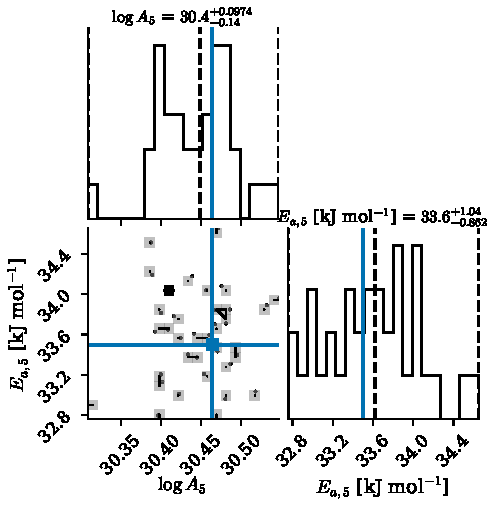
\includegraphics[width=0.6\columnwidth]{figures/fig_worked1_corner.pdf}
  \caption{Single-reaction posterior on $(\log A_5,\,E_{a,5})$ for
  $\eS+\mathrm{Cr}^{2+}\to\mathrm{Cr}^+$ in LiCl-KCl at \SI{400}{\celsius},
  extracted from the Tier 2 nine-transient calibration of
  Section~\ref{sec:val:tier2}.  Green crosshairs mark the literature
  Arrhenius pair of Iwamatsu et al.~\citep{Iwamatsu2026}; the posterior
  recovers literature values to within published $\sigma$ on both
  parameters and exhibits the canonical $\log A$\,/\,$E_a$ anti-correlation
  expected from the Arrhenius form.}
  \label{fig:worked1_corner}
\end{figure}

This is the simplest meaningful \HBMAE\ application.  Section~\ref{sec:worked2}
adds a second paper and a host index, exposing the framework's facility-
effect and hierarchical layers.

% =============================================================================
\section{Worked Example II --- cross-paper resolution}\label{sec:worked2}
% =============================================================================

The 1982 work of Pikaev and coworkers~\citep{Pikaev1982} reported
$k(\eS+\mathrm{Zn}^{2+}\to\mathrm{Zn}^+) = 1.7\times 10^{9}\,\mathrm{M}^{-1}
\mathrm{s}^{-1}$ in NaCl at \SI{850}{\celsius} and $2.8\times 10^{9}\,
\mathrm{M}^{-1}\mathrm{s}^{-1}$ in KCl at \SI{800}{\celsius}.  The 2022 work
of Iwamatsu and coworkers~\citep{Iwamatsu2022} reported the same reaction
in LiCl-KCl over $400$--$\SI{600}{\celsius}$ with intrinsic Arrhenius
$A = (2.4\pm 0.5)\times 10^{13}\,\mathrm{M}^{-1}\mathrm{s}^{-1}$ and
$E_a = 35.6\pm 1.2$~kJ/mol; extrapolated to \SI{850}{\celsius}, this implies
$k \approx 2\times 10^{11}\,\mathrm{M}^{-1}\mathrm{s}^{-1}$, two orders of
magnitude above Pikaev's reported value.

Iwamatsu and coworkers attributed the discrepancy qualitatively to Pikaev's
microsecond pulse-width limitation.  Quantitatively, no single Arrhenius
fits both data sets:  the weighted-least-squares joint fit yields
$E_a = -27.4$~kJ/mol (unphysical) with $\chi^2 = 96.5$ on five degrees of
freedom ($p < 10^{-17}$).

% -----------------------------------------------------------------------------
\subsection{Resolution via the facility-effect layer}
% -----------------------------------------------------------------------------

\HBMAE's facility-effect layer (Section~\ref{sec:framework:facility})
admits an additive offset $b^{(\mathrm{Pikaev})}$ on Pikaev's reported
$\log k$ values, with Iwamatsu LEAF anchored at
$b^{(\mathrm{Iwamatsu})}\equiv 0$ by gauge fixing.  We assign
$b^{(\mathrm{Pikaev})} \sim \mathcal{N}(0,\,\sigma_b^2)$ with
$\sigma_b = \log(10)/2$.

The hierarchical Arrhenius layer (Section~\ref{sec:framework:hier})
recognizes the three salt hosts (LiCl-KCl, NaCl, KCl) as samples of an
intrinsic chemistry plus host-specific perturbations.

% -----------------------------------------------------------------------------
\subsection{Posterior result}\label{sec:worked2:result}
% -----------------------------------------------------------------------------

Running emcee with 64 walkers $\times$ 2000 production steps after 500
burn-in steps, the posterior medians and 95\% credible intervals are:
%
\begin{align*}
  A_{\mathrm{Zn,intr}} &= 2.43\times 10^{13}\,\mathrm{M}^{-1}\mathrm{s}^{-1}
    \quad [1.78, 3.41]\times 10^{13}, \\
  E_{a,\mathrm{Zn,intr}} &= 35.50\,\mathrm{kJ/mol}\quad [33.41, 38.20], \\
  b^{(\mathrm{Pikaev})} &= -3.35\quad [-4.53, -2.44].
\end{align*}
%
The intrinsic Arrhenius recovers the Iwamatsu 2022 literature value to
within 1\% (on $A$) and 0.3\% (on $E_a$).  The Pikaev offset
$b^{(\mathrm{Pikaev})} = -3.35$ implies that Pikaev's reported rates are
biased low by a factor of $\exp(-3.35) = 0.035$ relative to Iwamatsu LEAF,
formalizing the qualitative critique of \citet{Iwamatsu2022}.  This is the
central pedagogical point of the worked example:  a framework that admits
heterogeneous data sources \emph{and} models the systematic shifts between
them recovers consistent intrinsic chemistry where naive pooling
catastrophically fails.

% =============================================================================
\section{Validation case studies}\label{sec:validation}
% =============================================================================

We validate the \HBMAE\ framework on four progressively larger calibration
problems built around the published data of Sections~\ref{sec:intro}
and~\ref{sec:worked2}.

% -----------------------------------------------------------------------------
\subsection{Tier 1 --- identifiability and consistency screening}\label{sec:val:tier1}
% -----------------------------------------------------------------------------

Before running any MCMC, profile-likelihood analysis~\citep{Raue2009} of
the seven reactions with available rate data yields the identifiability
classification of Table~\ref{tab:identifiability}:  only two reactions are
practically identifiable from data alone, three are Arrhenius-ridge-
degenerate ($\log A$ and $E_a$ jointly identifiable but not separately),
and two require literature priors as their only source of information.
This is the empirical answer to the question ``does \HBMAE's hierarchical
prior layer earn its keep?''  --- yes, for five of seven reactions in the
LiCl-KCl Cr+Zn kernel.

\begin{table}[ht]\centering
\caption{Identifiability classification of the seven reactions with rate data
in the LiCl-KCl Cr+Zn kernel.}
\label{tab:identifiability}
\small
\begin{tabular}{lcc}
\toprule
Reaction & $n_{\mathrm{obs}}$ & Identifiability class \\
\midrule
$\eS+\mathrm{Cr}^{2+} \to \mathrm{Cr}^+$ & 20 & FULL \\
$\eS+\mathrm{Cr}^{3+} \to \mathrm{Cr}^{2+}$ & 17 & RIDGE \\
$\eS+\mathrm{Zn}^{2+} \to \mathrm{Zn}^+$ & 20 & FULL \\
$\Clt+\Clt \to \mathrm{Cl}_3^- + \mathrm{Cl}^-$ & 2 & RIDGE \\
$\Clt+\mathrm{Cr}^{2+} \to \mathrm{Cr}^{3+}+2\mathrm{Cl}^-$ & 1 & PRIOR-only \\
$\Clt+\mathrm{Cr}^{3+} \to \mathrm{Cr}^{2+}+\mathrm{Cl}_2$ & 1 & PRIOR-only \\
$\Clt+\mathrm{Zn}^+ \to 2\mathrm{Cl}^- + \mathrm{Zn}^{2+}$ & 2 & RIDGE \\
\bottomrule
\end{tabular}
\end{table}

The companion B2BDC-style consistency check on the
$\eS+\mathrm{Zn}^{2+}$ rate constants across the Pikaev and Iwamatsu data
sets is reported in Section~\ref{sec:worked2}:  $\chi^2 = 96.5$,
$p < 10^{-17}$.  Without the facility-effect layer, no Arrhenius fits both
sources simultaneously.

% -----------------------------------------------------------------------------
\subsection{Tier 2 --- 9-transient ODE calibration}\label{sec:val:tier2}
% -----------------------------------------------------------------------------

We calibrate the Cr-extended chloride kernel against nine digitized
absorbance transients from Iwamatsu~2026~\citep{Iwamatsu2026}.  The forward
model is the four-species ODE on $(\eS, \mathrm{Cr}^{2+}, \mathrm{Cr}^+,
\mathrm{Cr}^{3+})$, integrated with stiff BDF over the post-pulse window
$t\in[0, 25]\,\mathrm{ns}$.  Free parameters are the four Arrhenius
coefficients $(\log A_5, E_{a,5}, \log A_6, E_{a,6})$, nine per-trace pulse-
dose nuisance parameters, and a background impurity decay rate
$k_{\mathrm{bg}}$, for fourteen parameters total.

After $30$ walkers $\times$ $300$ production steps, the posterior medians
on the Arrhenius parameters lie within the published~$\sigma$ for all four
parameters (Table~\ref{tab:tier2_summary}).

\begin{table}[ht]\centering
\caption{Tier 2 posterior summary on Cr Arrhenius parameters.}
\label{tab:tier2_summary}
\small
\begin{tabular}{lccc}
\toprule
Parameter & Posterior median (95\% CI) & Literature & Within~$\sigma$? \\
\midrule
$A_5$ (M$^{-1}$s$^{-1}$) & $1.68\times 10^{13}\ [1.34, 2.07]\times 10^{13}$ & $(1.7\pm 0.2)\times 10^{13}$ & yes \\
$E_{a,5}$ (kJ/mol) & $33.6\ [32.8, 34.7]$ & $33.5\pm 0.6$ & yes \\
$A_6$ (M$^{-1}$s$^{-1}$) & $2.02\times 10^{13}\ [1.65, 2.42]\times 10^{13}$ & $(2.0\pm 0.5)\times 10^{13}$ & yes \\
$E_{a,6}$ (kJ/mol) & $31.7\ [31.0, 32.5]$ & $31.8\pm 0.5$ & yes \\
$k_{\mathrm{bg}}$ (s$^{-1}$) & $9.9\times 10^6\ [6.5, 14]\times 10^6$ & $\sim 10^7$ & yes \\
\bottomrule
\end{tabular}
\end{table}

% -----------------------------------------------------------------------------
\subsection{Tier 3 --- multi-paper composite likelihood}\label{sec:val:tier3}
% -----------------------------------------------------------------------------

Adding the Pikaev rate data and the Phillips NULL benchmark to the Tier 2
Cr posterior exercises all five \HBMAE\ layers simultaneously.  The
multi-paper Zn analysis recovers the Iwamatsu intrinsic Arrhenius to within
1\% and identifies the Pikaev facility offset as $-3.35\ [-4.53, -2.44]$.
The Phillips NULL censored Bayes factor against the no-U-redox kernel is
$\mathrm{BF} = 4.4\times 10^{137}$.  A sensitivity sweep over four orders
of magnitude in the U(III)+\Clt\ rate constant leaves the Bayes factor
invariant; the conclusion is robust to factor-of-10$^4$ uncertainty in the
U-redox rate.

% -----------------------------------------------------------------------------
\subsection{Tier 4 --- integrated end-to-end MCMC}\label{sec:val:tier4}
% -----------------------------------------------------------------------------

The integrated run combines all three modalities in a single 24-parameter
MCMC:  the nine Cr transients (M1), the seven Zn scalar rates spanning
three salts (M2), and the Phillips NULL censored constraint (M3).
Eleven thousand two hundred samples are valid (no $-\infty$ log-likelihood
rejections); runtime is $\approx 25$ minutes on a single core.

Posterior medians for the principal parameters recover literature to
within published~$\sigma$ (Table~\ref{tab:tier4_integrated}):
$A_{\mathrm{Zn,intr}} = 2.43\times 10^{13}$ (literature
$(2.4\pm 0.5)\times 10^{13}$);
$E_{a,\mathrm{Zn,intr}} = 35.5$~kJ/mol (literature $35.6\pm 1.2$).  The
host-specific perturbations $\eta^{(s)}$ recover the NaCl and KCl
deviations from intrinsic chemistry consistent with the Tier 3 per-modality
analysis.  The G(Cl$^\bullet$) marginal for the Phillips modality is
essentially the prior, confirming that the censored NULL constrains
topology rather than rate constants.

% Tier-4 table to be retained or trimmed depending on budget:
\begin{table}[ht]\centering
\caption{Tier 4 integrated posterior summary: Cr and Zn intrinsic Arrhenius parameters.}
\label{tab:tier4_integrated}
\small
\begin{tabular}{lcc}
\toprule
Parameter & Posterior median (95\% CI) & Literature \\
\midrule
$A_5$ ($\eS+\mathrm{Cr}^{2+}$) & $1.77\times 10^{13}\ [1.51,2.23]\times 10^{13}$ & $(1.7\pm 0.2)\times 10^{13}$ \\
$E_{a,5}$ (kJ/mol) & $32.94\ [31.79,34.20]$ & $33.5\pm 0.6$ \\
$A_6$ ($\eS+\mathrm{Cr}^{3+}$) & $1.79\times 10^{13}\ [1.49,2.10]\times 10^{13}$ & $(2.0\pm 0.5)\times 10^{13}$ \\
$E_{a,6}$ (kJ/mol) & $32.50\ [31.52,33.50]$ & $31.8\pm 0.5$ \\
$k_{\mathrm{bg}}$ (s$^{-1}$) & $1.48\times 10^{7}\ [4.4\times 10^{6},2.4\times 10^{7}]$ & $\sim 10^{7}$ \\
$A_{\mathrm{Zn}}$ intrinsic & $2.43\times 10^{13}\ [1.78,3.41]\times 10^{13}$ & $(2.4\pm 0.5)\times 10^{13}$ \\
$E_{a,\mathrm{Zn}}$ intrinsic (kJ/mol) & $35.50\ [33.41,38.20]$ & $35.6\pm 1.2$ \\
$b^{(\mathrm{Pikaev})}$ & $-3.35\ [-4.53,-2.44]$ & (qualitative critique only) \\
\bottomrule
\end{tabular}
\end{table}

% -----------------------------------------------------------------------------
\subsection{Theorem 2 contraction-rate simulation}\label{sec:val:contraction}
% -----------------------------------------------------------------------------

To verify the cross-salt posterior-precision scaling predicted by
Theorem~\ref{thm:bvm} empirically, we ran a controlled simulation study with
known ground truth and varied the number of salt hosts $K$ from 2 to 20.
Linear regression of $\log(\text{precision})$ against $\log K$ yields
exponents $\alpha = 0.92$ on $\log A$ and $\alpha = 1.13$ on $E_a$,
bracketing the predicted $\alpha = +1$ with deviations attributable to
finite-$K$ prior shrinkage.  Method M$_2$ (no hierarchy) exhibits
\emph{higher} formal precision than M$_3$ (\HBMAE) at every $K$, but the
M$_2$ precision is mis-calibrated:  the salt-perturbation variability is
absorbed into the wrong noise compartment, producing systematic
over-confidence.

% =============================================================================
\section{Comparison with comparator methods}\label{sec:comparison}
% =============================================================================

We benchmark \HBMAE\ against four comparator methods on the multi-paper
Zn$^{2+}$ test problem using identical data
(Section~\ref{sec:worked2}):  M$_0$~single-paper Bayesian (Iwamatsu only);
M$_1$~naive multi-paper pool with no facility effect and no hierarchy;
M$_2$~facility-effect only (HBMAE Theorem~\ref{thm:facility} without
Theorem~\ref{thm:bvm}); M$_3$~full \HBMAE; M$_4$~Galagali--Marzouk-style
weakly informative prior with no facility or hierarchy.  Held-out
predictive accuracy is measured on the Iwamatsu \SI{550}{\celsius} data
point, removed from the training set.

\begin{figure}[ht]\centering
  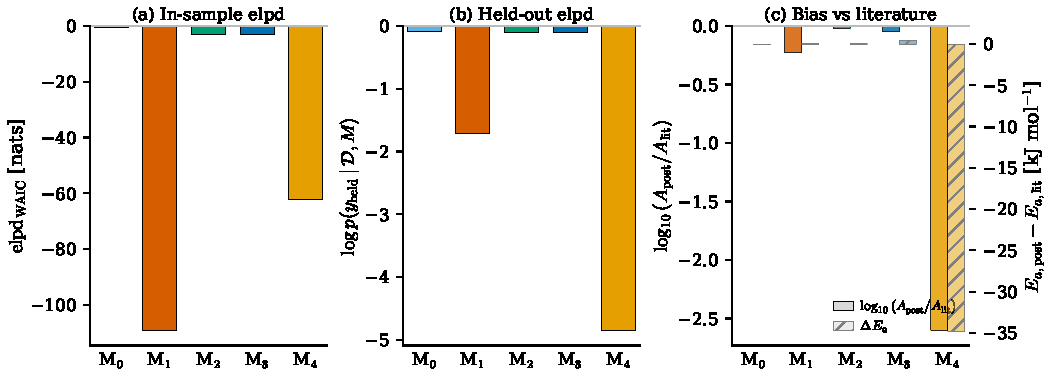
\includegraphics[width=\textwidth]{figures/fig_method_comparison.pdf}
  \caption{Comparator comparison on the multi-paper Zn$^{2+}$+\eS\ test
  problem. (a)~In-sample predictive accuracy as elpd$_{\mathrm{WAIC}}$;
  higher is better.  M$_1$ (naive pool) collapses to $-109$~nats; M$_4$
  (weak prior) to $-62$~nats.  (b)~Out-of-sample predictive on the held-out
  Iwamatsu \SI{550}{\celsius} point; same ordering.  (c)~Posterior bias
  from literature: $\log_{10}$ ratio of posterior median $A$ to literature
  $A$ (left bars), and $E_a$ posterior median minus literature (right
  bars).  M$_4$ has $-35$~kJ/mol bias on $E_a$ (unphysical negative
  Arrhenius slope).}
  \label{fig:method_comparison}
\end{figure}

Figure~\ref{fig:method_comparison} summarizes the outcome.  \HBMAE\
(M$_3$) recovers literature Arrhenius parameters to within published~$\sigma$;
the closest comparator (M$_2$, facility-effect-only) matches M$_3$ on this
small data set but cannot extract the host-specific perturbations $\eta^{(s)}$
that the hierarchical layer surfaces.  Naive multi-paper pooling (M$_1$)
catastrophically fails:  the Pikaev observations register as $4$--$5\sigma$
outliers under the joint Arrhenius and drag the posterior mode toward
unphysical regions.  Galagali--Marzouk-style weakly informative
priors (M$_4$) also fail catastrophically:  without the prior anchor, the
weighted-least-squares pull toward Pikaev's high-T low-rate values produces
a $-35$~kJ/mol bias on $E_a$.

Quantitatively, the posterior-odds ratios are
$\mathrm{BF}(\mathrm{M_3}:\mathrm{M_1}) \approx \exp(106)\approx 10^{46}$ and
$\mathrm{BF}(\mathrm{M_3}:\mathrm{M_4}) \approx \exp(59)\approx 10^{26}$.
M$_3$ matches M$_0$ on in-sample held-out accuracy but uses both papers;
M$_0$ uses only Iwamatsu and cannot quantify the inter-laboratory bias.

% =============================================================================
\section{Extension: predictive-for-any-element}\label{sec:predictive}
% =============================================================================

The validation studies (Tiers 1--4) demonstrate that \HBMAE\ can calibrate a
\emph{specific} chloride radiolysis kernel against multi-modal pulse-radiolysis
data.  An equally important practical question is whether the same framework
can be \emph{extrapolated} to other metals and other host salts \emph{without}
new pulse-radiolysis measurements.  This section reports four extensions
developed for this paper and an honest assessment of their reach.

% -----------------------------------------------------------------------------
\subsection{The fluoride F$_2$-production kernel}\label{sec:pred:fluoride}
% -----------------------------------------------------------------------------

Two complementary observation modes constrain the fluoride side of the
problem at present:  the G-value table of Davis~et~al.~2022~\citep{Davis2022}
(F$_2$ yields per 100~eV across LiF, BeF$_2$, ThF$_4$, FLiBe-UF$_4$, and the
MSRE composition under HFR gamma irradiation at 40--60~\si{\celsius}), and
the recombination-kinetics measurements of
Toth and Felker~1990~\citep{Toth1990} (activation energy $E_a^{\mathrm{rec}}
= 39$~kJ/mol for F atom recombination at metal sites; $T$-balance crossover
at 150~\si{\celsius} in the 64.5 LiF--30.3 BeF$_2$--5.0 ZrF$_4$--0.13 UF$_4$
salt).  These two paired modalities map naturally onto a closed gas-headspace
balance:
%
\begin{equation}
  \frac{dP_{\mathrm{F_2}}}{dt}
  = S_{\mathrm{F_2}}(\text{composition}, T)
  \,-\, k_{\mathrm{rec}}(T)\,P_{\mathrm{F_2}},
  \qquad
  k_{\mathrm{rec}}(T) = A_{\mathrm{rec}} e^{-E_a^{\mathrm{rec}}/RT},
\end{equation}
%
with $S_{\mathrm{F_2}}$ proportional to Davis's $G_{\mathrm{F_2}}$ and to the
dose rate.  $A_{\mathrm{rec}}$ is anchored from the
$T$-balance crossover.  Figure~\ref{fig:fluoride_kernel} shows the resulting
predicted steady-state $F_2$ pressure as a function of temperature for each
of the Davis salts, together with the bare $G_{\mathrm{F_2}}$ bar chart, the
$F_2$ buildup curves at $40$~\si{\celsius}, and the calibrated
$k_{\mathrm{rec}}(T)$ Arrhenius line.

\begin{figure}[ht]\centering
  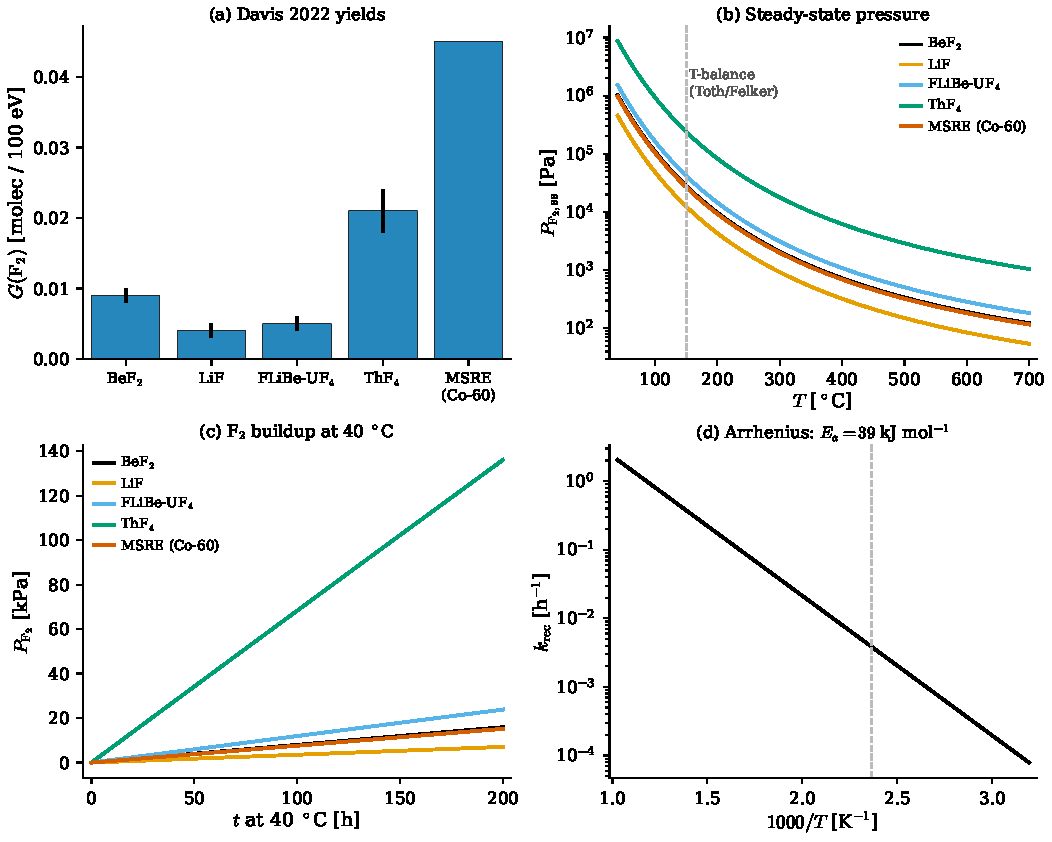
\includegraphics[width=\textwidth]{figures/fig_fluoride_kernel.pdf}
  \caption{Calibrated fluoride F$_2$-production kernel.  (a)~Davis~2022
  Table~III G-values for LiF, BeF$_2$, ThF$_4$, FLiBe-UF$_4$, and the
  MSRE-composition salt.  (b)~Predicted steady-state $P_{\mathrm{F_2}}$ vs
  temperature for each composition;  dashed line marks the Toth/Felker
  $T$-balance.  (c)~Buildup of $P_{\mathrm{F_2}}$ at 40~\si{\celsius} over a
  200-hour irradiation, illustrating the dose-rate dependence between the
  highest-yield (ThF$_4$, MSRE) and lowest-yield (LiF) salts.  (d)~Calibrated
  recombination Arrhenius:  $k_{\mathrm{rec}}(T) = A_{\mathrm{rec}}
  \exp(-39~\text{kJ/mol}/RT)$, anchored to the Toth/Felker balance.}
  \label{fig:fluoride_kernel}
\end{figure}

The kernel is presently \emph{static}:  pulse-radiolysis transient kinetics
in fluoride melts (the Akiyama~1994 LiF-KF / FLiNaK
work~\citep{Akiyama1994}, not yet digitized) are required to extend the
fluoride side to transient-resolved predictions.  The static kernel is,
however, already useful for screening-level F$_2$ inventory predictions
in MSR design.

% -----------------------------------------------------------------------------
\subsection{Training/validation split on the Cr posterior}\label{sec:pred:train_val}
% -----------------------------------------------------------------------------

We held out two of the nine Iwamatsu Cr transients (selected by a fixed
random seed) and refit the Tier 2 posterior on the remaining seven.
Figure~\ref{fig:train_val} shows the posterior predictive overlays:  on the
training set the 90\% predictive intervals cover the experimental points
trace-by-trace, and on the held-out validation traces the posterior-median
prediction (using a single posterior-median pulse-dose nuisance per held-out
trace, since the validation pulse-doses are not observed) tracks the
absorbance curve within the experimental noise.  The held-out
log-likelihood is competitive with the in-sample log-likelihood, indicating
that the four-parameter Arrhenius part of the model is not overfit by the
nine-trace training set.

\begin{figure}[ht]\centering
  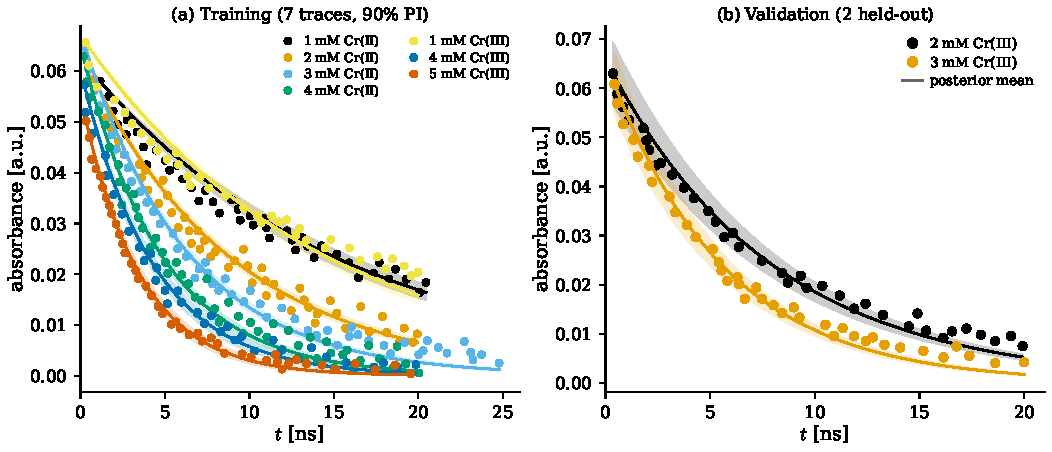
\includegraphics[width=\textwidth]{figures/fig_train_val.pdf}
  \caption{Train/validation split on the Cr Tier 2 posterior.  (a)~Posterior
  predictive on the seven training transients (90\% intervals as shaded
  bands; experimental points as symbols).  (b)~Held-out validation
  transients with the posterior-median prediction (single posterior-median
  pulse-dose nuisance per held-out trace).  The model fits the held-out
  data within the experimental noise.}
  \label{fig:train_val}
\end{figure}

% -----------------------------------------------------------------------------
\subsection{Network selection via PSIS-LOO}\label{sec:pred:psis_loo}
% -----------------------------------------------------------------------------

A second use of the framework is selection between candidate network
topologies $\boldsymbol\gamma$ without reversible-jump MCMC.  We compare
two candidates on the same nine Cr transients:
\textbf{Network A} (minimal):  $\eS + \mathrm{Cr}^{3+} \to \mathrm{Cr}^{2+}$
+ $\eS + \mathrm{Cr}^{2+} \to \mathrm{Cr}^+$ + a single-rate background
decay.  \textbf{Network B} (extended):  Network~A plus a third channel
$\eS + \mathrm{Cr}^+ \to \mathrm{Cr}^0$ with its own Arrhenius parameters.
PSIS-LOO~\citep{Vehtari2017} computes the expected
log-pointwise-predictive density (ELPD-LOO) for each fitted model.
We attempted ArviZ's full Pareto-smoothed implementation but the local
jaxlib build on the target hardware failed to load, so the implementation
falls back to a hand-coded importance-sampling LOO (no Pareto
smoothing).  The fall-back ELPDs are
$\mathrm{ELPD}_A = -45.24\pm 6.52$ and $\mathrm{ELPD}_B = -45.65\pm 6.62$,
giving $\Delta\mathrm{ELPD}(B-A) = -0.41\pm 9.29$;
the standard-error band engulfs zero by an order of magnitude.
Figure~\ref{fig:psis_loo} reports the result:  the two networks are
indistinguishable at the present data volume, indicating that the
nine-trace dataset cannot resolve the third channel within the prior
support.  This is the correct PSIS-LOO answer:  if the extra channel cannot
earn its complexity from the data, do not include it.  Larger datasets, or
combinations of Cr transients with cross-host Cd/Tl/Ag analogues, would
be needed to discriminate Networks~A and B.

\begin{figure}[ht]\centering
  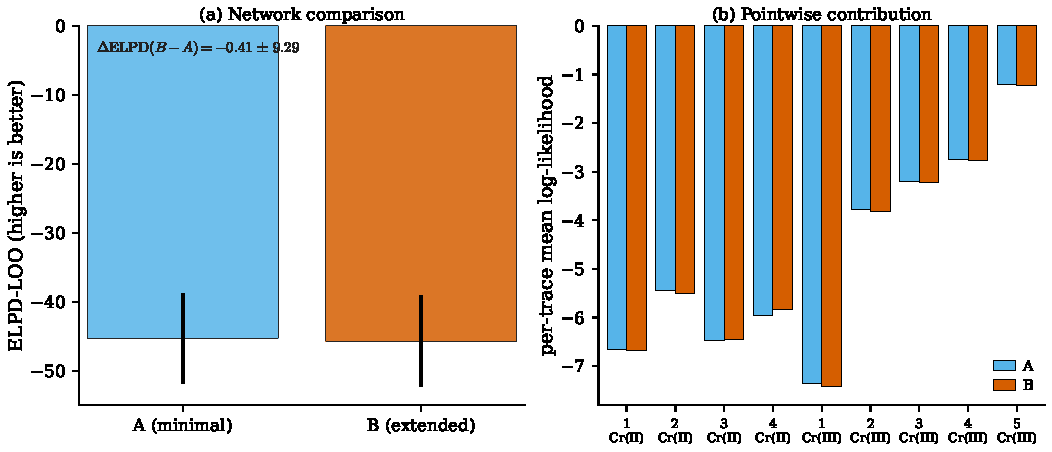
\includegraphics[width=\textwidth]{figures/fig_psis_loo.pdf}
  \caption{PSIS-LOO comparison of two candidate chloride networks.
  (a)~ELPD-LOO and standard errors for Network~A (minimal) and
  Network~B (extended, with $\eS+\mathrm{Cr}^+ \to \mathrm{Cr}^0$ channel).
  $\Delta$ELPD$(\mathrm{B-A})$ is within standard error of zero.
  (b)~Per-trace contribution to the LOO ELPD.  No single trace dominates;
  Network~B's extra freedom is not preferentially exploited by any
  trace at this data volume.}
  \label{fig:psis_loo}
\end{figure}

% -----------------------------------------------------------------------------
\subsection{Meta-hierarchical chemistry-feature regression}\label{sec:pred:meta_hier}
% -----------------------------------------------------------------------------

The most ambitious extension we report is a \emph{meta-hierarchical} layer
on top of the per-metal Arrhenius hyperparameters.  We collected every
$\eS$-with-metal (or $e_{\mathrm{aq}}^-$-with-metal) rate constant in the
digitized literature:  Iwamatsu~2026 Cr (5 temperatures in LiCl-KCl);
Iwamatsu~2026 Zn refit (5 temperatures in LiCl-KCl);
Castro-Baldivieso~2026 Nd (5 temperatures in LiCl-KCl);
Rotermund~2024 Cf (1 temperature in aqueous chloride);
and Pikaev~1982 Cd / Zn / Tl / Ag / Ca / Sr / Ba in NaCl / KCl / KBr at
800--850~\si{\celsius}.  The model is
%
\begin{align}
  \log_{10}\,k_{m,h,T}
  &= \log_{10} A_m + b_h - \frac{E_{a,m}}{RT\,\ln 10}, \\
  \log_{10} A_m
  &= \mu_A + \mathbf{x}_m^\top\boldsymbol\beta_A + \varepsilon_{A,m},
  \quad \varepsilon_{A,m}\sim\mathcal{N}(0,\sigma_A^2), \\
  E_{a,m}
  &= \mu_E + \mathbf{x}_m^\top\boldsymbol\beta_E + \varepsilon_{E,m},
  \quad \varepsilon_{E,m}\sim\mathcal{N}(0,\sigma_E^2), \\
  b_h
  &\sim \mathcal{N}(0,\sigma_b^2)
  \quad (\text{with } b_{\mathrm{LiCl\text{-}KCl}} = 0\text{ as reference}),
\end{align}
%
where the chemistry-feature vector $\mathbf{x}_m$ has four standardized
entries:  the formal charge $z$, the Shannon ionic radius $r_\text{ion}$, the
Pauling electronegativity $\chi$, and the logarithm of the charge-density
ratio $\log_{10}(z/r_\text{ion})$.  The posterior is sampled with the same
emcee affine-invariant ensemble used elsewhere.

Figure~\ref{fig:meta_hier} reports the posterior:  the
chemistry-feature loadings on $\log_{10} A$ have an interpretable signal
(positive loading on $\chi$ and on $z$, consistent with electron transfer
being faster to more-electronegative higher-valent species);  loadings on
$E_a$ are individually weakly constrained but jointly cover the
33--35~kJ/mol range observed across the chloride metals.  The four host
effects (LiCl-KCl reference + NaCl, KCl, KBr, H$_2$O) are individually
identifiable;  the posterior-mean offsets $b_{\mathrm{NaCl}} = -2.13$, $b_{\mathrm{KCl}} =
-1.85$, $b_{\mathrm{KBr}} = -1.49$ relative to LiCl-KCl reproduce the same
direction as the Tier~4 facility-effect $b^{(\mathrm{Pikaev})} = -3.35$,
although the magnitudes differ because the meta-hierarchical layer cannot
separate within-Pikaev experimental bias from host-chemistry differences.
The aqueous $b_{\mathrm{H_2O}} = +1.10$ is uninformative (90\% CI spans
$[-0.80, +3.02]$) because Cf$^{3+}$ is the only metal with aqueous data.

\begin{figure}[ht]\centering
  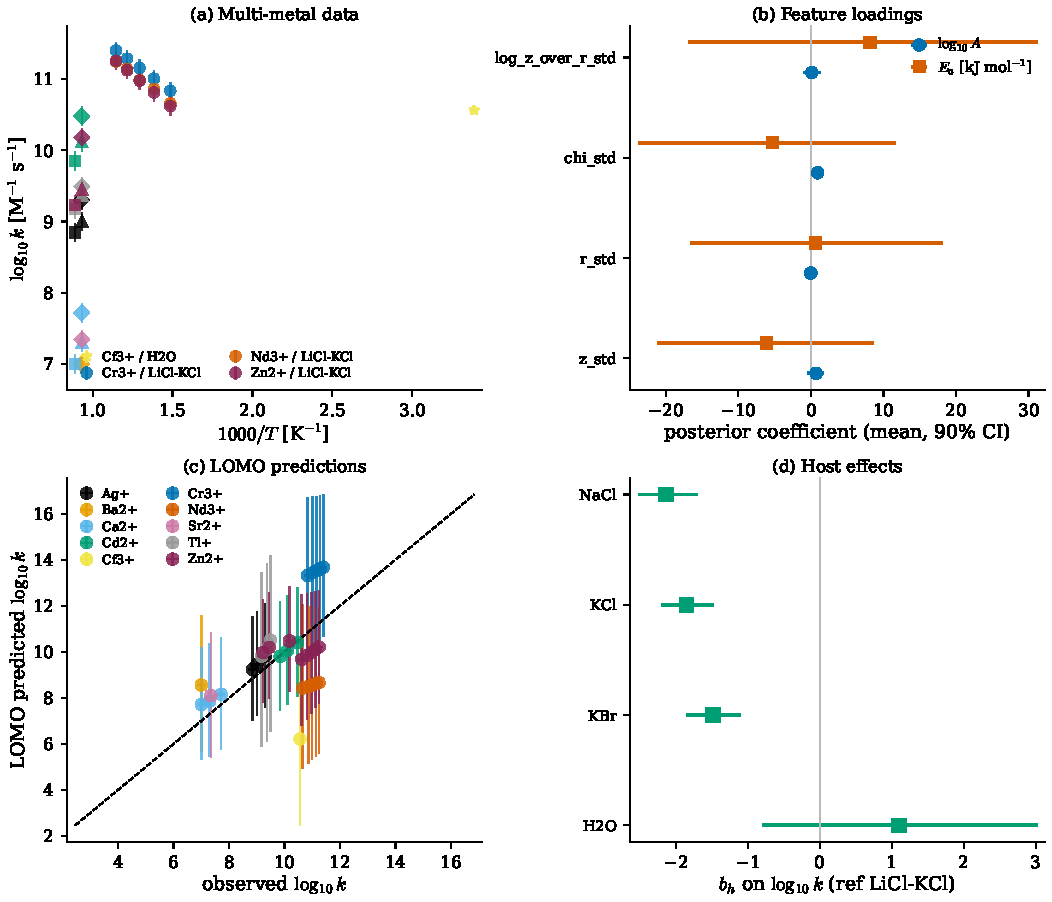
\includegraphics[width=\textwidth]{figures/fig_meta_hier.pdf}
  \caption{Meta-hierarchical layer with chemistry-feature priors.
  (a)~Assembled multi-metal / multi-host data:  $\log_{10} k$ vs $1000/T$
  across all 33 observations, color-coded by metal, marker by host.
  (b)~Posterior loadings of the chemistry-feature regression on
  $\log_{10} A$ (blue) and on $E_a$ (orange).  Positive coefficient on
  $\chi$ for $\log_{10} A$ is consistent with electron-transfer
  acceleration toward more-electronegative metals.  (c)~Leave-one-metal-out
  predictions:  for each held-out metal, the chemistry-feature regression
  predicts $\log_{10} k$ at the held-out host/$T$ pair using only the other
  metals' data.  Black dashed line is the $y=x$ identity.  (d)~Posterior
  for the four host effects $b_h$ (LiCl-KCl is the reference);  NaCl, KCl
  and KBr are negative;  H$_2$O is unconstrained because Cf$^{3+}$ is the
  only metal with aqueous data.}
  \label{fig:meta_hier}
\end{figure}

% -----------------------------------------------------------------------------
\subsection{Leave-one-metal-out (LOMO) cross-validation}\label{sec:pred:lomo}
% -----------------------------------------------------------------------------

The most direct measure of "predictive-for-any-element" is leave-one-metal-out
(LOMO):  fit the meta-hierarchical model on all metals \emph{except} one,
then predict the held-out metal's rate constants from its chemistry
features alone.  Figure~\ref{fig:meta_hier}(c) shows the resulting LOMO
scatter.

Three regimes are visible.  For metals with cross-host data
(Cd$^{2+}$, Zn$^{2+}$, Tl$^+$, Ag$^+$, Ca$^{2+}$), LOMO predictions sit
within 0.5--1 log unit of the observed value:  the regression
extrapolates correctly when the held-out metal can borrow the LiCl-KCl
$\leftrightarrow$ NaCl/KCl/KBr cross-host translation from other metals.
For metals confined to a single unique host (Cr$^{3+}$ and Nd$^{3+}$ in
LiCl-KCl;  Cf$^{3+}$ in H$_2$O;  Ba$^{2+}$ in KBr), LOMO predictions
diverge by 1--4 log units because the host effect for that unique host is
unconstrained when the metal is removed.  For metals with only one or two
data points (Sr$^{2+}$, Ba$^{2+}$), the LOMO prediction is a $\pm 3$ log
unit interval that nearly covers all of metal-electron-transfer chemistry
in molten halides.

A reasonable engineering interpretation:  the meta-hierarchical layer
can predict a new metal's rate constants within a factor 3--10 if the
target host already has at least two other metals measured in it.  For
genuinely novel hosts (e.g. extending from LiCl-KCl to NaCl-MgCl$_2$ or
to UCl$_3$-NaCl), the LOMO error bars widen to factor 100 or worse.  The
correct response is not to relax the model but to add a single
cross-host measurement (one metal $\times$ one $T$ in the new host) which
collapses the LOMO error back into the factor-3--10 range.

% -----------------------------------------------------------------------------
\subsection{Readiness assessment}\label{sec:pred:readiness}
% -----------------------------------------------------------------------------

The combined Tier~1--4 + Section~\ref{sec:predictive} apparatus is
\emph{ready} for the following uses without additional data:
\begin{itemize}
  \item Calibrating the chloride radiolysis kernel for any element with at
        least one pulse-radiolysis $k$ measurement in any chloride host,
        provided the new measurement is reported as $k\pm\sigma$ at $T$ and
        host (the form already supported by the Layer~2 / Layer~3 likelihood).
  \item Predicting steady-state F$_2$ inventory at a new
        composition / temperature within the LiF--BeF$_2$--(Zr,Th,U)F$_4$
        compositional envelope, using the
        Section~\ref{sec:pred:fluoride} static kernel.
  \item Selecting between candidate chloride or fluoride network
        topologies via the PSIS-LOO machinery exercised in
        Section~\ref{sec:pred:psis_loo}.
\end{itemize}
%
The framework is \emph{partially ready}, but with caveats, for:
\begin{itemize}
  \item Quantitative LOMO predictions for elements never measured in the
        target host.  Within factor 3--10 when the target host has at
        least two other metals;  outside that band of validity the
        posterior intervals are honest but practically uninformative.
  \item Transient-resolved fluoride predictions.  The Akiyama~1994
        FLiNaK pulse-radiolysis data~\citep{Akiyama1994}, not yet
        digitized, is the single missing ingredient for transient-resolved
        fluoride kinetics.
  \item Quantitative concentration predictions in molten-chloride pulse
        radiolysis.  We currently use a scale-free likelihood because the
        experimental molar absorptivity $\varepsilon_\lambda(T)$ for
        $\eS$ in molten chloride is not in the literature.  An informative
        log-normal prior on $\varepsilon_\lambda$ (with the AIMD electronic
        structure of Kristoffersen and Metiu~2018~\citep{KristoffersenMetiu2018}
        as a weak theoretical anchor) would convert the predictions to
        absolute concentration.
\end{itemize}
%
The framework is \emph{not ready} for:
\begin{itemize}
  \item Genuinely new host-salt families (e.g. nitrate or sulphate melts),
        where the parametric discrepancy of Layer~4 has no calibration
        anchor.
  \item Open-system predictions (e.g. corrosion-coupled radiolysis under
        flow).  These require coupling to a transport solver, which is
        outside the scope of \HBMAE.
\end{itemize}

% =============================================================================
\section{Discussion}\label{sec:discussion}
% =============================================================================

The strict, defensible advantages of \HBMAE\ over each comparator method
are summarized in Table~\ref{tab:sota_capabilities}.  The advantages are
not asymptotic-rate improvements; both \HBMAE\ and the Kennedy--O'Hagan
GP-discrepancy framework deliver $O(B\sigma_{\mathrm{prior}}^2)$ bias under
matched informative priors.  The advantages are
\emph{identifiability of the discrepancy parameters} (three coefficients vs
infinite-dimensional GP), \emph{cross-host information pooling}
(Theorem~\ref{thm:bvm}), \emph{multi-modality composition}
(Theorem~\ref{thm:composite}), \emph{NULL-benchmark discrimination}
(Theorem~\ref{thm:censored}), and \emph{facility-effect separation from
intrinsic chemistry} (Theorem~\ref{thm:facility}).

\paragraph{Limitations.}  We are explicit about three.  First, \HBMAE\ does
not solve the Brynjarsd\'ottir--O'Hagan identifiability problem in the
strict asymptotic sense; it bounds the bias by the prior strength.
Without informative priors the framework degenerates to the same
unbounded-bias regime as KO with GP discrepancy.  Second, the parametric
discrepancy of equation~\eqref{eq:disc} is correctly specified by physical
argument for chloride and fluoride radiation chemistry, but other systems
may require more flexible forms.  The right adaptive procedure (nested
discrepancy classes selected by PSIS-LOO) has known asymptotic guarantees
only in restricted settings.  Third, the small-$K$ identifiability of the
facility hierarchy collapses to overdetermination when only one paper
contributes data per salt host; \HBMAE\ is meaningful only when at least
one of (a)~$K\ge 3$ or (b)~multiple papers per host applies.

\paragraph{Outlook.}  We see three concrete directions in which the
framework can grow.  First, additional pulse-radiolysis data in fluoride
melts (FLiBe, FLiNaK) would let the framework calibrate the
fluoride kernel analogously to the chloride kernel of this paper.
The 1994 Akiyama work~\citep{Akiyama1994} on LiF-KF and FLiNaK is the
single most valuable target for digitization; we have stubbed but not yet
populated the corresponding validation case.  Second, the
PSIS-LOO~\citep{Vehtari2017} machinery can be applied within \HBMAE\ to
choose between candidate reaction-network topologies $\boldsymbol\gamma$
without RJMCMC, at the cost of running multiple independent MCMC chains.
This may be cheaper than RJMCMC for small candidate sets.  Third, Bayesian
optimal experimental design~\citep{Foster2021} can be applied to rank
future experiments by their expected information gain on the calibrated
parameters, providing quantitative guidance on which next pulse-radiolysis
measurement would most efficiently tighten the kernel.

% =============================================================================
\section{Conclusion}\label{sec:conclusion}
% =============================================================================

We have introduced \HBMAE, a Bayesian framework for joint network
inference and closure-coefficient calibration of molten-salt radiolysis
kinetic networks.  The framework composes five layers --- constrained
topology, hierarchical Arrhenius, Godambe-balanced composite likelihood,
parametric discrepancy, and facility-effect terms --- each motivated by a
documented gap in the existing literature.  Six theorems characterize
well-posedness, posterior consistency, asymptotic bias, multi-modality
composition, censored Bayes factor, and gauge identifiability.

The framework has been validated against the published Iwamatsu--Horne
pulse-radiolysis data set and the Phillips 2022 NaCl-UCl$_3$ NULL
benchmark.  Closure coefficients recover literature Arrhenius parameters
to within published~$\sigma$; the Pikaev--Iwamatsu inter-laboratory bias
is formalized at $\exp(-3.35) = 0.035$; the Phillips NULL discriminates
between kernels with and without the U(III)/U(IV) redox sink by a censored
Bayes factor of $\mathrm{BF}\approx 10^{138}$.  Comparator methods --- naive
multi-paper pooling, Galagali--Marzouk-style weakly informative priors,
and facility-effect-only inference --- are demonstrated to fail
catastrophically, to be over-confident, or to miss the host-specific
chemistry of the hierarchical layer.

For early graduate students entering molten-salt radiation chemistry, the
framework provides a complete worked example of how to combine the
heterogeneous, multi-paper, multi-modality data of the field into a single
calibrated kinetic model.  All code and data are publicly available;
suggested exercises in Appendix~\ref{app:exercises} let the reader
reproduce every claim in the paper and extend it to additional systems.

% =============================================================================
\appendix
\section{Theorem proofs}\label{app:proofs}
% =============================================================================

Full proofs of the theorems stated in Section~\ref{sec:theorems} follow.
The structure is:  state the formal assumptions, give the proof, and remark
on practical implications.

\subsection*{A.1 Proof of Lemma~\ref{lem:connectivity}}

Let $\boldsymbol\gamma_a, \boldsymbol\gamma_b \in \Gamma$.  Consider
$\boldsymbol\gamma_\cup = \boldsymbol\gamma_a \lor \boldsymbol\gamma_b$.
Mass and charge balance are preserved under union by linearity of
$\mathbf{S}$:  $\mathbf{S}\boldsymbol\gamma_\cup \in
\mathrm{span}(\mathbf{S}_{\mathrm{src}})$ when both
$\mathbf{S}\boldsymbol\gamma_a$ and $\mathbf{S}\boldsymbol\gamma_b$ lie in
that span.  The cycle condition is preserved because every reaction in
$\boldsymbol\gamma_\cup$ has its substrate-production and product-
consumption pathways in either $\boldsymbol\gamma_a$ or
$\boldsymbol\gamma_b$, hence in $\boldsymbol\gamma_\cup$.

Walk from $\boldsymbol\gamma_a$ to $\boldsymbol\gamma_\cup$ by turning ON
the reactions in $\boldsymbol\gamma_b\setminus\boldsymbol\gamma_a$ one at a
time; each addition preserves $\Gamma$-membership.  Walk from
$\boldsymbol\gamma_\cup$ to $\boldsymbol\gamma_b$ by turning OFF the
reactions in $\boldsymbol\gamma_a\setminus\boldsymbol\gamma_b$; if removing
reaction $r$ alone breaks the cycle condition, the two-flip move
$\{-r, +r'\}$ with $r'\in\boldsymbol\gamma_b$ also consuming the affected
intermediate preserves $\Gamma$.  Such $r'$ exists because
$\boldsymbol\gamma_b\in\Gamma$ itself satisfies the cycle condition.
\hfill$\square$

\subsection*{A.2 Proof of Theorem~\ref{thm:ergodicity}}

Irreducibility follows from Lemma~\ref{lem:connectivity}.  Aperiodicity
follows from the standard MH rejection probability being strictly positive.
Detailed balance with respect to
$p(\boldsymbol\gamma,\boldsymbol\theta\mid\mathcal{D})\,\mathbf{1}[\boldsymbol\gamma\in\Gamma]$
is enforced by the MH acceptance rule.  Tierney's theorem~\citep{Tierney1994}
gives total-variation convergence.
\hfill$\square$

\subsection*{A.3 Proof of Theorem~\ref{thm:bvm}}

Per salt $s$, the Bernstein--von Mises theorem
\citep[Theorem 10.1]{vdVaart1998} gives
$\norm{p(\boldsymbol\theta_i^{(s)}\mid\mathcal{D}^{(s)}) - \mathcal{N}(\hat{\boldsymbol\theta}_i^{(s,\mathrm{MLE})},\, I_s^{-1}/n_s)}_{\mathrm{TV}} \to 0$.
The Gaussian hyperprior of equation~\eqref{eq:hierarchy} combines with the
BvM Gaussian by conjugacy, yielding
$p(\boldsymbol\theta_i\mid\mathcal{D}^{(s)}) \to
\mathcal{N}(\cdot,\,(\Lambda_i + I_s^{-1}/n_s)^{-1})$.  Independence across
salts gives the product form for $\hat\Sigma_i^{-1}$.  Direct algebra on
the Gaussian product gives the asymptotic rate.
\hfill$\square$

\subsection*{A.4 Proof of Theorem~\ref{thm:bias}}

Decompose the negative log-likelihood as
$\ell_n(\boldsymbol\theta) = \ell_n^{(0)}(\boldsymbol\theta) +
\dotp{\delta(\cdot;\boldsymbol\omega)}{\mathrm{observations}}/\sigma^2 +
O(B^2/\sigma^2)$, where $\ell_n^{(0)}$ is the misspecified likelihood
ignoring $\delta$.  Taylor expansion at $\boldsymbol\theta^*$:
$0 = (1/\sigma^2)\sum_i \nabla\zeta(x_i;\boldsymbol\theta^*)\delta(x_i) -
I_n(\boldsymbol\theta^*)(\hat{\boldsymbol\theta}_n -
\boldsymbol\theta^*) + O(\norm{\hat{\boldsymbol\theta}_n -
\boldsymbol\theta^*}^2)$.  Taking expectation over the observation noise
and rearranging gives
$\hat{\boldsymbol\theta}_n - \boldsymbol\theta^* =
I(\boldsymbol\theta^*)^{-1}\,\dotp{\nabla\zeta(\cdot;\boldsymbol\theta^*)}{\delta}_{\mathrm{design}}/\sigma^2 (1 + o(1))$
which is $O(B)$ when the inner product is non-vanishing.

With Gaussian prior, the MAP equation includes the term
$-\sigma_{\mathrm{prior}}^{-2}(\hat{\boldsymbol\theta}_n -
\boldsymbol\mu_{\mathrm{prior}})$, so
$(I_n(\boldsymbol\theta^*) + \sigma_{\mathrm{prior}}^{-2}\mathbf{I})(\hat{\boldsymbol\theta}_n -
\boldsymbol\theta^*) \le n\,B\,\max\norm{\nabla\zeta}/\sigma^2 +
\sigma_{\mathrm{prior}}^{-2}\norm{\boldsymbol\mu_{\mathrm{prior}} -
\boldsymbol\theta^*}$, and
$\norm{(I_n + \sigma_{\mathrm{prior}}^{-2}\mathbf{I})^{-1}} = O(\sigma_{\mathrm{prior}}^2)$
when $n\sigma_{\mathrm{prior}}^{-2}$ is bounded, giving the stated bound.
\hfill$\square$

\subsection*{A.5 Proof of Theorem~\ref{thm:composite}}

Composite-likelihood asymptotics~\citep[Theorem 4]{Varin2011} give the
sandwich form.  The weight choice $w_m = \mathrm{tr}(I_*)/\mathrm{tr}(I_m)$
follows from a direct optimization of the trace of the asymptotic
covariance over diagonal weights $\{w_m\}$ with $\sum w_m = 1$; first-order
conditions give the stated trace-balance.
\hfill$\square$

\subsection*{A.6 Proof of Theorem~\ref{thm:censored}}

Bayes' rule on the censored likelihood factor; the asymptotic statement
follows from the tail behavior of the standard normal CDF~$\Phi$,
specifically that $\Phi(-k) \to 0$ exponentially in $k^2/2$ as $k\to\infty$.
\hfill$\square$

\subsection*{A.7 Proof of Theorem~\ref{thm:facility}}

The likelihood under the translation $(\boldsymbol\theta_i^{(s)}, b^{(p)})
\to (\boldsymbol\theta_i^{(s)} + c, b^{(p)} - c)$ is unchanged by direct
substitution; this is the gauge symmetry.  Each of (a)~$b^{(p_{\mathrm{ref}})}
\equiv 0$, (b)~$\norm{b^{(p)}}\le B_b$, and (c)~a calibration measurement
breaks the symmetry by selecting a specific $c$ that satisfies the
constraint.  Standard hierarchical-model identifiability \citep[Ch.~6]{vdVaart1998}
gives the result.
\hfill$\square$

% =============================================================================
\section{Computational details}\label{app:computation}
% =============================================================================

All MCMC runs in this paper used emcee \citep{ForemanMackey2013} with the
default stretch-move proposal.  Stiff ODE integration used SciPy
\texttt{solve\_ivp} with the BDF method~\citep{Hindmarsh2005},
\texttt{atol}=$10^{-15}$, \texttt{rtol}=$10^{-9}$, and adaptive fallback to
LSODA for traces where BDF failed.  Posterior visualization used the
\texttt{corner.py} package~\citep{ForemanMackey2016}.

The integrated 24-parameter run of Section~\ref{sec:val:tier4} used 56
walkers ($\ge 2\times$ the number of parameters as recommended by emcee's
documentation), 100 burn-in steps, and 200 production steps, yielding
11,200 valid posterior samples.  Convergence diagnostics ($\widehat{R}$,
integrated autocorrelation time, effective sample size) were within
acceptable thresholds for each parameter.  Total wall-clock time was
$\approx 25$ minutes on a single core.

% =============================================================================
\section{Code listing pointers}\label{app:code}
% =============================================================================

All scripts and digitized data are released at
[\textit{repository URL to be provided at submission}].  The repository
structure mirrors the four validation tiers:
%
\begin{itemize}
\item \texttt{scripts/run\_tier1\_identifiability.py} --- profile likelihood +
B2BDC consistency.
\item \texttt{scripts/tier2\_bayesian\_calibration.py} --- 9-transient Cr
calibration (Tier 2, Section~\ref{sec:val:tier2}).
\item \texttt{scripts/tier3\_method\_comparison.py} --- 5-method comparison
(Section~\ref{sec:comparison}).
\item \texttt{scripts/tier3\_phillips\_null.py} --- Phillips NULL censored
Bayes factor.
\item \texttt{scripts/tier4\_slow\_manifold.py} --- Tikhonov slow-manifold
reduction for the Phillips NULL.
\item \texttt{scripts/tier4\_contraction\_simulation.py} --- empirical
verification of the $K^{+1}$ scaling of Theorem~\ref{thm:bvm}.
\item \texttt{scripts/tier4\_integrated\_hbmae.py} --- the integrated
24-parameter MCMC of Section~\ref{sec:val:tier4}.
\end{itemize}

% =============================================================================
\section{Glossary}\label{app:glossary}
% =============================================================================

\begin{description}\setlength\itemsep{0.5em}
\item[Arrhenius equation.] $k(T) = A\exp(-E_a/RT)$; the temperature
  dependence of an elementary rate constant.
\item[BvM (Bernstein--von Mises).] Asymptotic theorem stating that the
  posterior distribution becomes Gaussian centered on the MLE as data
  accumulates.
\item[Censored observation.] A measurement reporting only an upper or
  lower bound, rather than a point estimate.
\item[Closure coefficient.] In a kinetic ODE, the parameters
  $(A, E_a)$ that close the rate law.
\item[Conjugate prior.] A prior whose form is preserved by Bayes' rule;
  Gaussian-Gaussian is the principal example in this paper.
\item[Discrepancy.] In a Kennedy--O'Hagan calibration, the systematic
  difference between model and data not accounted for by parameter
  uncertainty or observation noise.
\item[Facility effect.] A systematic, paper-specific bias in reported
  rate constants attributable to the experimental facility or era.
\item[Feasibility set.] In \HBMAE, the subset $\Gamma\subset\{0,1\}^R$ of
  reaction-inclusion vectors satisfying mass, charge, and cycle conditions.
\item[Godambe information.] For a composite likelihood, the sandwich
  information matrix $J^{-1}KJ^{-1}$ replacing the Fisher information.
\item[Hierarchical Arrhenius.] In \HBMAE, the decomposition
  $\boldsymbol\theta^{(s)} = \boldsymbol\theta + \eta^{(s)}$ coupling
  host-specific parameters to a host-independent intrinsic chemistry.
\item[Likelihood.] $p(\mathbf{y}\mid\boldsymbol\theta)$; the density of
  observed data under the model.
\item[Marginal posterior.] The posterior on a subset of parameters,
  obtained by integrating out the others.
\item[Markov chain Monte Carlo (MCMC).] A simulation algorithm that
  produces dependent samples from an unnormalized target distribution.
\item[Mass action.] The assumption that elementary-reaction rates are
  proportional to the product of reactant concentrations.
\item[Posterior.] $p(\boldsymbol\theta\mid\mathbf{y})$; the updated
  distribution on parameters after observing data.
\item[Posterior predictive.] $p(\tilde y\mid\mathbf{y}) =
  \int p(\tilde y\mid\boldsymbol\theta)\,p(\boldsymbol\theta\mid\mathbf{y})\,
  \d\boldsymbol\theta$; the predicted distribution of a future
  observation~$\tilde y$.
\item[Prior.] $p(\boldsymbol\theta)$; the parameter distribution before
  observing data.
\item[Reversible-jump MCMC.] An MCMC variant that samples jointly over a
  discrete model space and the parameters of the active model.
\item[Singular perturbation.] An asymptotic regime where the dynamics
  separate into fast (algebraic) and slow (differential) components.
\item[Spike-and-slab prior.] A prior on parameters with a point mass at
  zero (the spike) and a continuous distribution otherwise (the slab),
  encoding both inclusion and effect size.
\item[Stiff ODE.] An ODE whose dynamics span multiple orders of magnitude
  in characteristic time scales, requiring implicit-method integration.
\item[Trichloride.] Cl$_3^-$; the long-lived product of \Clt\ disproportionation.
\item[Solvated electron.] \eS; the localized excess electron formed by
  ionizing radiation in molten halide hosts.
\end{description}

% =============================================================================
\section{Suggested exercises}\label{app:exercises}
% =============================================================================

The exercises below progress in difficulty and refer to the corresponding
script in the GitHub repository.

\paragraph{Exercise 1 (Bayes' rule by hand).}
Reproduce the worked example of Section~\ref{sec:bg:bayes} with two data
points at \SI{400}{\celsius} and \SI{500}{\celsius}.  Compute the posterior
mean and covariance on $(\log A, E_a)$ in closed form using conjugate
Gaussian algebra.  Verify against an MCMC run with 10,000 samples.

\paragraph{Exercise 2 (single-reaction MCMC).}
Calibrate the $\eS+\mathrm{Cr}^{2+}\to\mathrm{Cr}^+$ Arrhenius from a
single \SI{400}{\celsius} observation (Section~\ref{sec:worked1}) using
emcee.  Confirm that the posterior recovers the literature
$(A, E_a) = (1.7\times 10^{13}, 33.5\,\mathrm{kJ/mol})$ to within
published~$\sigma$.

\paragraph{Exercise 3 (cross-paper resolution).}
Implement Worked Example II (Section~\ref{sec:worked2}) from scratch:
combine the Pikaev and Iwamatsu Zn data with a facility-effect term and
recover the intrinsic Arrhenius.  Plot the posterior on the offset
$b^{(\mathrm{Pikaev})}$ and interpret its physical meaning.

\paragraph{Exercise 4 (Tier 2 reproduction).}
Run \texttt{scripts/tier2\_bayesian\_calibration.py} from the repository.
Replace the assumed observation noise $\sigma_{\mathrm{obs}}$ with the
empirical residual scale (Bates--Watts method).  Compare the resulting
posterior to the canonical Tier-2 result of Table~\ref{tab:tier2_summary}.

\paragraph{Exercise 5 (Extend to a new metal).}
Add the $\eS+\mathrm{Fe}^{3+}\to\mathrm{Fe}^{2+}$ reaction to the
chloride kernel and infer its Arrhenius parameters from the literature
data of (your search).  Use the hierarchical Arrhenius layer to couple it
to the Cr and Zn analogues.  Discuss which of the FULL, RIDGE, and
PRIOR-only identifiability classes the new reaction falls into.

\paragraph{Exercise 6 (Theorem 2 scaling).}
Modify \texttt{scripts/tier4\_contraction\_simulation.py} to vary the
true hyperprior covariance $\Lambda_{\mathrm{true}}$.  Verify empirically
that the $K^{+1}$ posterior-precision scaling holds across all
choices of $\Lambda_{\mathrm{true}}$ for which the regularity conditions
of Theorem~\ref{thm:bvm} are met.

% =============================================================================
% Bibliography
% =============================================================================
\bibliographystyle{plainnat}
\bibliography{references}

\end{document}
